\documentclass[en,license=none]{../../../eplsummary}

\usepackage{float}
\usepackage{../../../eplunits}
\usepackage[minted]{../../../eplcode}
\usepackage[english,ruled,vlined]{algorithm2e}


\graphicspath{{img/}}

\newcommand{\ipvf}{\textsc{ip}v4}
\newcommand{\ipvs}{\textsc{ip}v6}

% TODO add some figures

\hypertitle{Computer networks}{5}{INGI}{1341}
{Gilles Peiffer}
{Olivier Bonaventure}

\part{Principles}
\section{Connecting Two Hosts}
The first step when building a network,
even a worldwide network such as the Internet,
is to connect two hosts together.
In order for two hosts to exchange information,
they need to be linked by some kind of physical medium.
Various types of media have been used for this purpose:
\begin{itemize}
	\item \emph{Electrical cable}.
	Different types of cables are suitable for transmitting information:
	\begin{itemize}
		\item twisted pairs,
		which are used in the telephone network
		and in enterprise networks;
		\item coaxial cables,
		which are used in cable \textsc{TV} networks,
		but not in enterprise networks anymore.
	\end{itemize}
	Some technologies operate over the classical electrical cable.
	\item \emph{Optical fiber}.
	Optical fibers are used in networks
	when the distance between the devices is larger than one kilometer.
	There are two main types of optical fibers:
	\begin{itemize}
		\item multimode, which uses a \textsc{LED} to send signals
		over distances greater than several tens of kilometers;
		\item monomode, which uses a laser to send signals
		over distances of a few kilometers.
	\end{itemize}
	Both types can use repeaters to regenerate the signal
	and send it over another fiber.
	\item \emph{Wireless}.
	With this technology,
	a radio signal is used to encode the exchanged information.
	Modulation techniques are used
	to send information over a wireless channel.
	Some wireless networks use a laser
	that sends light pulses to a detector
	instead of a radio signal.
	These optical techniques allow to create point-to-point links,
	while radio based techniques can be used
	to build networks containing devices
	spread over a small geographical area.
\end{itemize}

\subsection{The Physical Layer}

The physical media explained previously can be used to exchange information,
once this information has been converted into a suitable electrical signal.
We will focus on the transmission of bits, i.e. either $0$ or $1$.

\begin{mydef}[Bit rate]
	In computer networks, the bit rate of the physical layer
	is always expressed in bits per second.
	This is in contrast with memory specifications
	which are usually expressed in bytes
	(one byte is equal to eight bits).
\end{mydef}

\subsubsection{Time-Sequence Diagram}

A physical transmission scheme
(interactions between communicating hosts)
can be described by using a \emph{time-sequence diagram}.
By convention, the sender is represented on the left,
and the receiver is on the right.
The middle of the diagram represents the electrical link.
Time flows from top to bottom.
To represent the transmission of a single bit,
three arrows are needed.
\begin{enumerate}
	\item The sender receives a request to transmit one bit of information.
	A \emph{primitive} is used to represent this request,
	sort of like a procedure call.
	The bit being transmitted is the only parameter.
	In the example in \figuref{timeseqdiag},
	the primitive is named \texttt{Data.request}.
	\item The dashed arrow indicates the signal's propagation time
	between the two hosts.
	Once the signal is received,
	it's interpreted and converted into a bit.
	\item The bit is delivered as a \texttt{Data.indication} primitive.
\end{enumerate}

\begin{figure}[H]
	\centering
	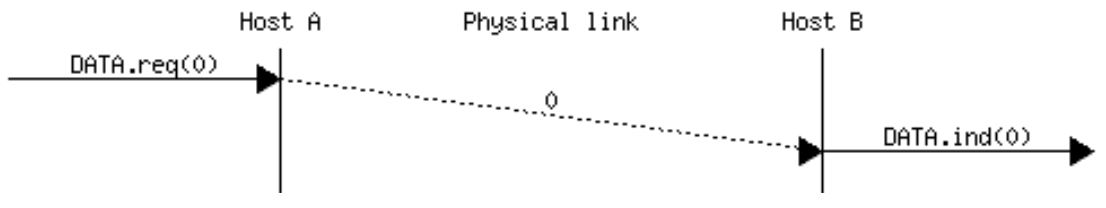
\includegraphics[width=0.5\textwidth]{timeseqdiag.png}
	\caption{A simple time-sequence diagram.}
	\label{fig:timeseqdiag}
\end{figure}

One of the problems of such a transmission scheme
is that electromagnetic interference can switch bits
while they're being transmitted
(i.e. a $0$ bit is sent but a $1$ bit is received).

With the above transmission scheme,
a bit is transmitted by setting the voltage on the electrical cable
to a specific value during some period of time.
One source of errors can be the difference in measured voltage
between the sender and the receiver.
Another reason could be that the two clocks do not operate
at exactly the same frequency.
Small differences in clock frequency imply
that bits can ``disappear'' or ``appear''
during their transmission on an electrical cable
(as in \figuref{lostbitdiag}).

\begin{figure}[H]
	\centering
	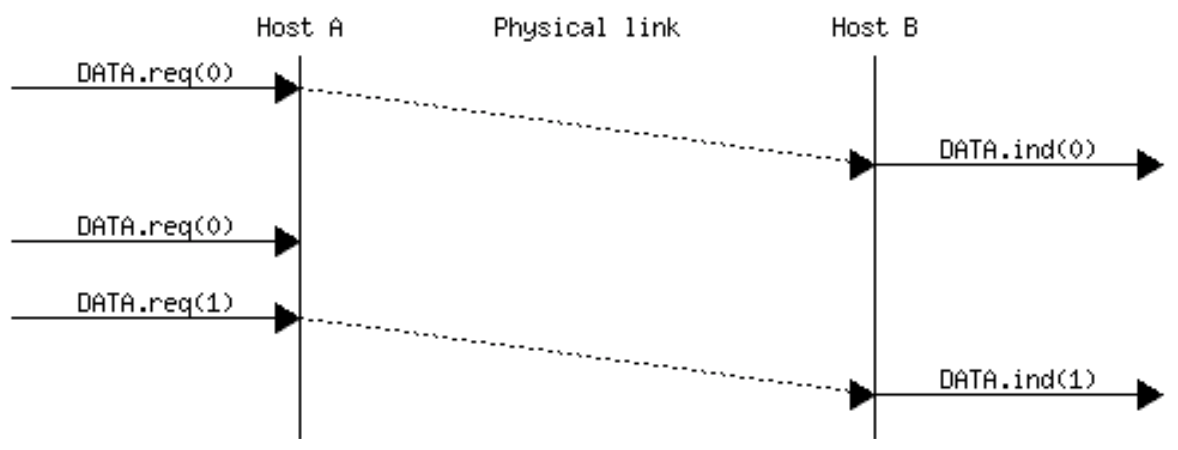
\includegraphics[width=0.5\textwidth]{lostbitdiag.png}
	\caption{Bits can ``disappear'' due to mismatched clock frequencies.}
	\label{fig:lostbitdiag}
\end{figure}

Due to these possible sources of error,
it's important to remember that the physical layer service may
\begin{itemize}
	\item \textbf{change} the value of a bit being transmitted,
	\item \textbf{deliver more (or less)} bits to the receiver
	than the bits sent by the sender.
\end{itemize}

\paragraph{Manchester Encoding} Other types of encodings have been defined
to transmit information over an electrical cable.
All physical layers are able to send and receive physical symbols
that represent the values $0$ and $1$.
However, for various reasons that are outside the scope of this chapter,
several physical layers exchange other physical symbols as well.
The Manchester encoding is an encoding scheme
in which time is divided into fixed-length periods.
Each period is divided into two halves
during which different voltage levels (high or low) can be applied.
The four possible combinations make for four possible characters,
as shown in \figuref{manchester_encoding}.

\begin{figure}[H]
	\centering
	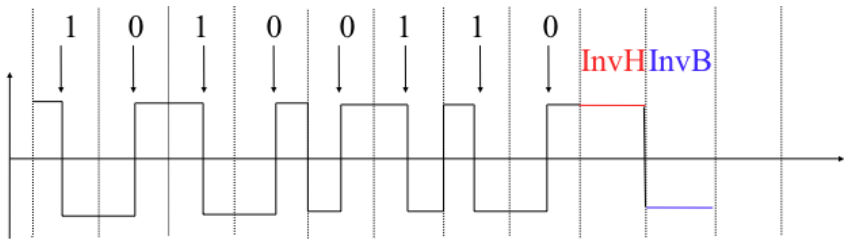
\includegraphics[width=\textwidth]{manchester_encoding.png}
	\caption{Visualisation of the Manchester encoding.
	$0$ and $1$ are regular bits,
	the InvH and InvB symbols can be used as markers
	for the beginning or end of frames.}
	\label{fig:manchester_encoding}
\end{figure}

\subsection{The Datalink Layer}

The physical layer is the name given
to all the functions related to the physical transmission of information.
It allows two or more entities to exchange bits
if they are connected to the same medium.
Computer networks use different layers,
where each layer provides a service that is built above the underlying layer,
and is close to the needs of the applications.
The datalink layer builds upon the service provided by the physical layer.
\bigbreak
\subsubsection{Framing}
\begin{mydef}[Frame]
	In many networks, the fundamental unit of of information
	exchanged between two hosts is called a \emph{frame}.
	A \emph{frame} is a sequence of bits
	that has a particular syntax or structure.
\end{mydef}
\begin{myrem}[Bit rate and bandwidth]
	Bit rate and bandwidth are often used
	to characterize the transmission capacity of the physical service.
	Bandwidth is defined as ``a range of radio frequencies
	which is occupied by a modulated carrier wave,
	which is assigned to a service,
	or over which a device can operate''.
	By extension, bandwidth is also used
	to represent the capacity of a communication system in bits per second.
\end{myrem}
Since the physical layer is not perfect,
transmitting and receiving frames
is not as simple as just defining a way to encode frames into bits,
or make out frames from bits.
A generic solution exists that works on any physical layer: \emph{stuffing}.
To enable a receiver to easily delineate the frame boundaries,
special bit strings serve as frame boundary markers
and encode the frames so that these special bit strings
do not appear inside the frames.
There are two variants of \emph{stuffing}:
\begin{itemize}
	\item \emph{Bit stuffing}.
	Bit stuffing reserves the $01111110$ bit string
	as the frame boundary marker
	and ensures there will never be six consecutive $1$ symbols
	transmitted by the physical layer inside a frame.
	It works as follows:
	\begin{enumerate}
		\item The sender transmits the marker, i.e. $01111110$.
		\item The sender sends all the bits of the frame
		and inserts an additional bit set to $0$
		after each sequence of five consecutive $1$ bits.
		\item The sender transmits the marker again,
		marking the end of the frame.
		\item The receiver detects the beginning of a frame
		thanks to the marker.
		\item The receiver processes the received bits,
		and if it counts five consecutive bits set to $1$,
		followed by a $0$ bit,
		that last bit is discarded.
		\item Once the receiver detects the marker again,
		it knows the frame has been received entirely.
	\end{enumerate}
	Bit stuffing increases the number of bits
	required to transmit the frame,
	with the worst case being
	a long sequence of bits set to $1$ inside the frame.
	Note that bit stuffing is vulnerable to transmission errors.
	If such an error happens,
	the frame (and possible the next)
	will not correctly be decoded by the receiver,
	but it will be able to resynchronize itself at the next valid marker.
	\item \emph{Character stuffing}.
	Character stuffing techniques
	use control characters in the \textsc{ASCII} table
	as markers to delineate frame boundaries.
	The following markers are often used:
	\textsc{DLE STX} to mark the beginning
	and \textsc{DLE ETX} to mark the end\footnote{\textsc{DLE} ($0010000$ b) for ``Data Link Escape'',
	\textsc{STX} ($0000010$ b) for ``Start of Text''
	and \textsc{ETX} ($0000011$ b) for ``End of Text''.}.
	When transmitting a frame,
	the sender adds a \textsc{DLE} character
	after each transmitted \textsc{DLE} character.
	This ensures that none of the markers
	can appear inside the transmitted frame.
	The receiver detects this
	and removes the second \textsc{DLE}
	when it receives two consecutive ones.
	Just like bit stuffing,
	character stuffing increases the length of the transmitted frames.
	The worst frame for character stuffing
	is a frame containing many \textsc{DLE} characters.
	Again, two frames can potentially be lost
	when a transmission error occurs,
	but the receiver will be able to resynchronize itself
	with the next correctly received markers.
\end{itemize}
While bit stuffing is easily implemented in hardware,
it is difficult to implement in software
given the complexity of performing bit manipulations in software.
Software implementations prefer to use character stuffing instead.

Both of these techniques allow to recover frames from a stream of bits or bytes.
The framing mechanism provides a richer service than the physical layer.
It can also be represented
using the \texttt{Data.req} and \texttt{Data.ind} primitives,
as illustrated in \figuref{stuffing_diag}.

\begin{figure}[H]
	\centering
	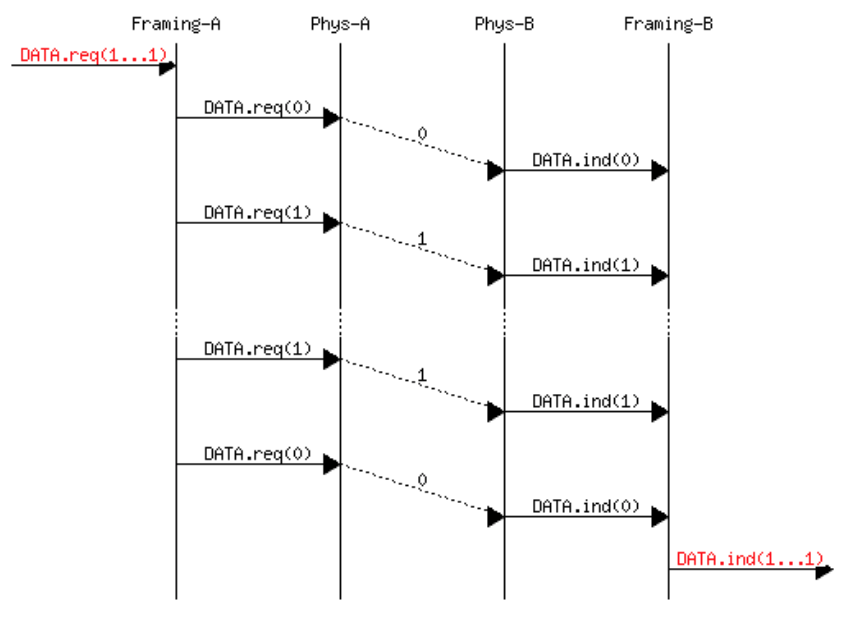
\includegraphics[width=0.4\textwidth]{stuffing_diag.png}
	\caption{Time-sequence diagram of framing,
	assuming hypothetical frames containing four useful bits
	and one bit of framing.}
	\label{fig:stuffing_diag}
\end{figure}

\subsubsection{Recovering From Transmission Errors}
We distinguish two types of \texttt{Data.req} and \texttt{Data.ind} primitives:
\begin{itemize}
	\item the interactions between the user and the datalink layer entity
	are represented using \texttt{Data.req} and \texttt{Data.ind};
	\item the interactions between the datalink layer entity
	and the framing sublayer
	are represented by using \texttt{send} and \texttt{recvd}.
\end{itemize}
The datalink layer entity has a buffer
to deal with \textsc{SDU}s\footnote{Service data unit,
a generic term to represent the data that is transported by a protocol.}
that have been received as a \texttt{Data.request}
but have not been sent.
It also has a buffer that deals with received frames
that haven't been processed yet.
If one of these buffers overflows,
arriving frames will be discarded,
even if they are correct.
Hence, a reliable protocol must include a feedback mechanism
that allows the receiver to inform the sender that it has processed a frame
and that another one can be sent,
regardless of transmission errors.
We need two types of frames:
\begin{itemize}
	\item \emph{data frames} carrying an \textsc{SDU};
	\item \emph{control frames} carrying an acknowledgment
	indicating the previous frames were processed correctly.
\end{itemize}
These two types can be distinguished by dividing the frame in two parts:
\begin{itemize}
	\item the \emph{header} that contains a bit
	set to $0$ in data frames and $1$ in control frames.
	\item the \emph{payload} that contains the \textsc{SDU}
	supplied by the application.
\end{itemize}
The datalink entity can then be modelled
as an \textsc{FSM}\footnote{Finite state machine.},
containing two states for the receiver and the sender (\figuref{fsm}).

\begin{figure}[H]
	\centering
	\begin{subfigure}[t]{0.45\linewidth}
		\centering
		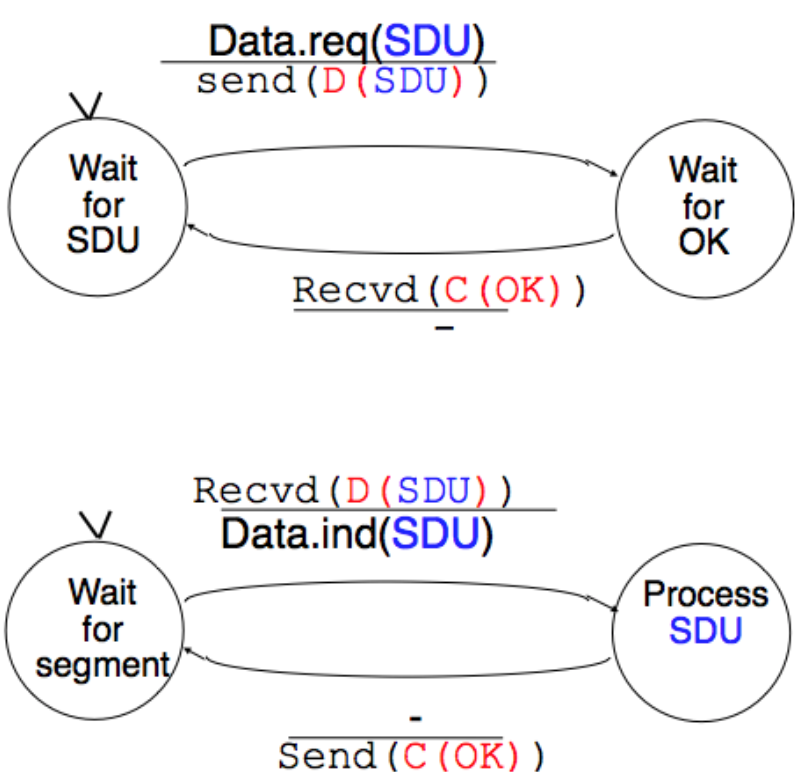
\includegraphics[width=0.6\textwidth]{fsm.png}
		\caption{\textsc{FSM} of the simplest reliable protocol,
		with the sender above and the receiver below.
		The sender has to wait for an acknowledgment
		before being able to transmit the next \textsc{SDU}.}
		\label{fig:fsm}
	\end{subfigure}
	\hfill
	\begin{subfigure}[t]{0.45\linewidth}
		\centering
		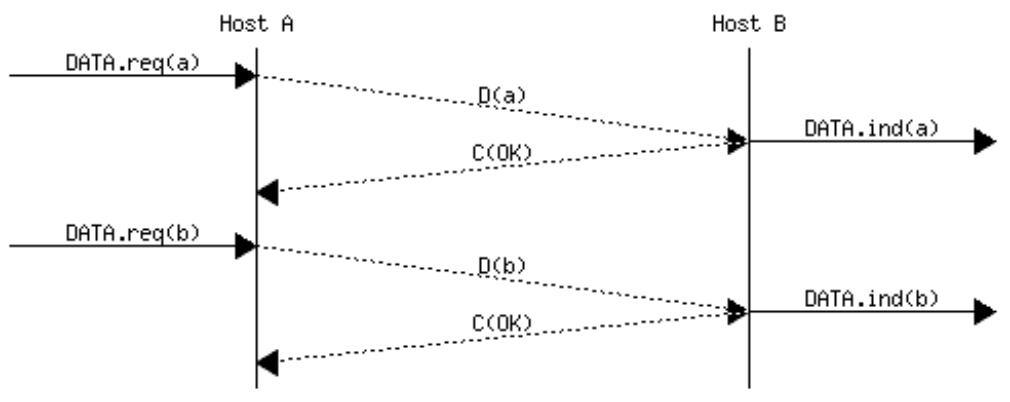
\includegraphics[width=\textwidth]{simp_rel_prot.png}
		\caption{Exchange of a few frames between two hosts.}
		\label{fig:simp_rel_prot}
	\end{subfigure}
\end{figure}

\subsubsection{Reliable Data Transfer On Top Of an Imperfect Link}
In the datalink layer,
we mainly have to deal with two types of transmission errors:
\begin{itemize}
	\item corrupted frames;
	\item lost or unexpected frames;
\end{itemize}
Data transmission on a physical link
can be affected by the following transmission errors:
\begin{itemize}
	\item random isolated errors
	where the value of a single bit has been modified;
	\item random burst errors
	where the values of $n$ consecutive bits have been changed;
	\item random bit creations and removals.
\end{itemize}
In order to avoid this,
we have to add \emph{redundancy} to the frames that are sent.
Information theory allows us to add redundant information
as an \emph{error detection code}.
Simply put,
the frame is sent with an error detection code,
computed by the sender, added to it.
Once the frame is received,
the receiver recomputes the error detection code
and verifies whether it matches the received one.
To understand error detection codes,
consider two devices that exchange bit strings containing $N$ bits.
To allow the receiver to detect a transmission error,
an error detection code calculates $r$ redundant bits
for each string of $N$ bits,
thus transforming the strings into strings of $N+r$ bits each.
The simplest error detection code is the parity bit.
Two types exist: even and odd parity.
With the even (resp. odd) parity scheme,
the redundant bit is chosen so that an even (resp. odd) number of bits
are set to $1$ in the transmitted string.
The receiver can easily recompute the parity of each received bit string
and discard the strings with an invalid parity.
This means that if multiple bits have been affected,
the receiver might not be able to detect the transmission error.
Another example of a (more powerful) error detection code
is a \textsc{CRC}\footnote{Cyclic redundancy check.},
which are widely used in datalink layer protocols.
\begin{myprop}[CRC]
	An $N$-bit \textsc{CRC} can detect
	\begin{itemize}
		\item all transmission errors affecting a burst
		of less than $N$ bits in the transmitted frame and
		\item all transmission errors that affect an odd number of bits.
	\end{itemize}
\end{myprop}

It is also possible to design a code
that allows the receiver to correct transmission errors,
the simplest example of which being
the \textsc{TMR}\footnote{Triple modular redundancy.},
where every bit is sent three consecutive times,
so as to allow the receiver to detect errors
and correct them by looking at the majority of bits in case an error occurs.
Other more powerful codes like the Hamming Code,
which is a clever combination of parity bits, exist.
However, these error correction schemes aren't really used in practice.

A frame is usually divided into two parts:
\begin{itemize}
	\item A \emph{header} that contains
	the fields used by the reliable protocol to ensure reliable delivery.
	The header contains a checksum or \textsc{CRC}
	that is used to detect transmission errors.
	Some headers also indicate a \emph{length field}
	with the length of the frame or the payload.
	\item A \emph{payload} that contains the user data.
\end{itemize}
The checksum is a simple error detection scheme:
both the sender and the receiver compute the arithmetic sum
of all the bytes of the frame.
Frames with an invalid checksum are discarded by the receiver.
\textsc{CRC}s have better error detection capabilities,
but require more processing power when implemented in software.
\begin{myrem}[Checksums and \textsc{CRC}s]
	Both checksums and \textsc{CRC}s are used in practice.
	The \textsc{TCP/IP} and \textsc{OSI} communities chose checksums
	(resp. the Internet checksum and the Fletcher checksum),
	while many datalink layer protocols and file formats such as
	\texttt{zip} or \texttt{png} use \textsc{CRC}s.
	It always comes down to a trade-off between error detection capabilities
	and processing power.
\end{myrem}

Since the receiver send an acknowledgment after each received data frame,
a retransmission timer is used.
The value of this retransmission timer needs to be larger
than the \textsc{RTT}\footnote{Round-trip time,
i.e. the delay between the transmission of the first bit of a data frame
to the reception of the last bit of the corresponding acknowledgment.}.
A retransmission timer is started when the sender sends a frame,
and when it expires,
the sender assumes the data segment was lost
and retransmits it (\figuref{retrans_timer}).
\begin{figure}[H]
	\centering
	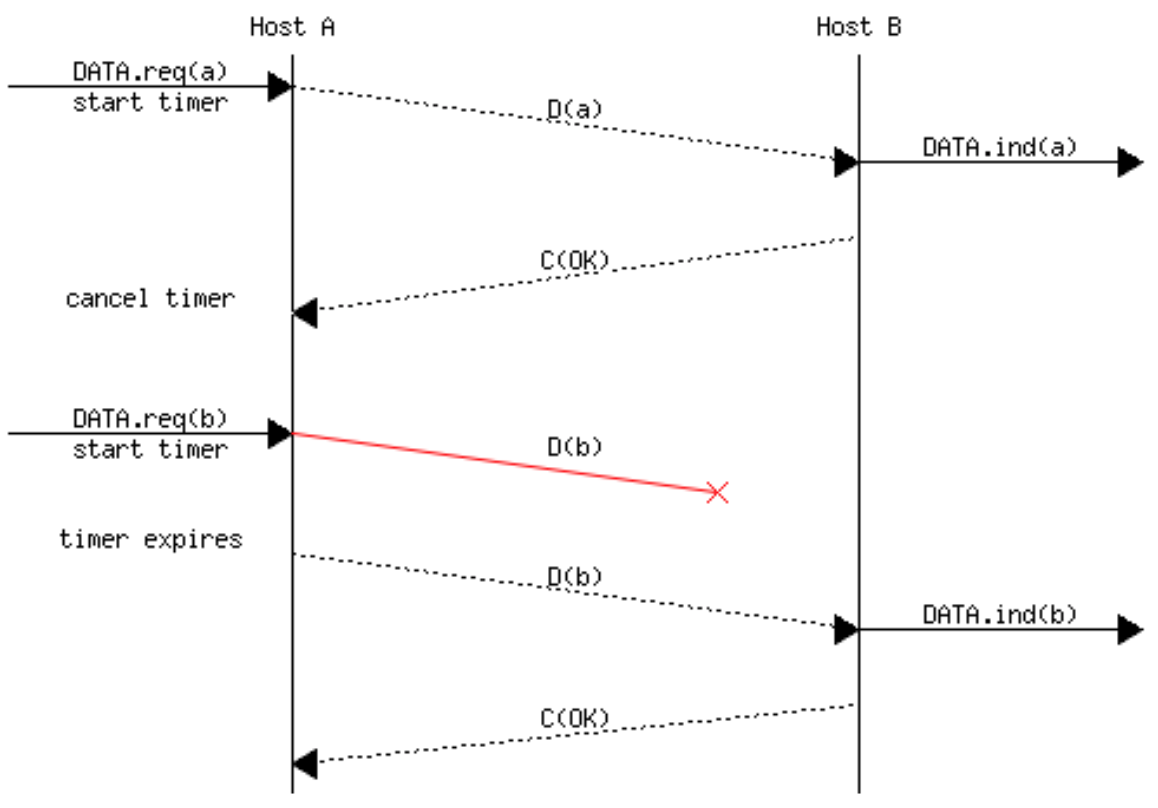
\includegraphics[width=0.4\textwidth]{retrans_timer.png}
	\caption{An example of retransmission timer expiry.}
	\label{fig:retrans_timer}
\end{figure}

However, an issue that can (and does) arise,
is the case when the acknowledgment is lost.
If this happens,
the sender will retransmit the data segment,
except that the receiver will interpret this retransmission as a new segment,
whose payload must be delivered to the user.
To solve this problem,
datalink protocols associate a seqnum\footnote{Sequence number.}
to each data frame.
This seqnum is one of the fields in the header of data frames.
We use the notation \texttt{D(x,\dots)}
to indicate a data frame whose seqnum field is set to value \texttt{x}.
The sequence number is encoded as a bit string of fixed length.
A simple reliable protocol
is \emph{Alternating bit protocol} (\textsc{ABP}).

\textsc{ABP} uses a single bit to encode the seqnum.
The sender and receiver
only require a four-state \textsc{FSM} (\figuref{abp_fsm}).

\begin{figure}[H]
	\centering
	\begin{subfigure}[t]{0.45\linewidth}
		\centering
		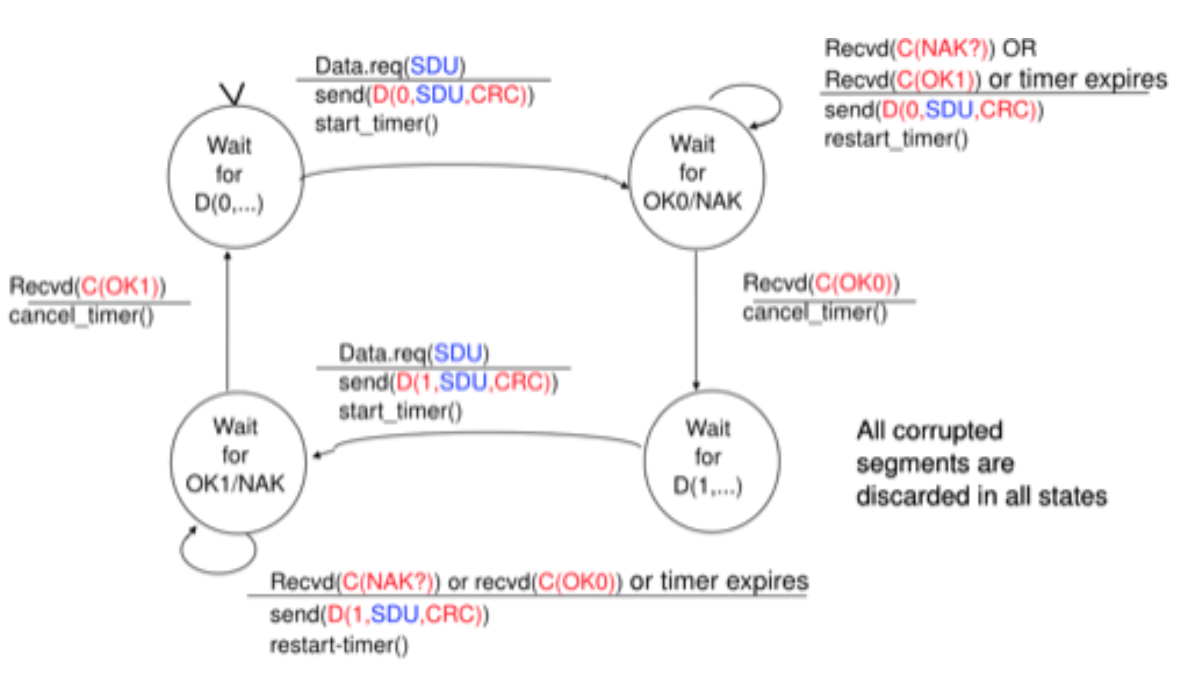
\includegraphics[width=\textwidth]{abp_sender_fsm.png}
		\caption{\textsc{ABP} sender \textsc{FSM}.
		The initial state of the sender
		is \texttt{Wait for D(0,\dots)}.
		In this state,
		the sender waits for a \texttt{Data.request}.
		The first data frame uses seqnum $0$.
		Once this is sent,
		the sender waits for an \texttt{OK0} acknowledgment.
		A frame is transmitted when the retransmission timer expires
		or when an acknowledgment with an incorrect seqnum
		has been received.}
		\label{fig:abp_sender_fsm}
	\end{subfigure}
	\hfill
	\begin{subfigure}[t]{0.45\linewidth}
		\centering
		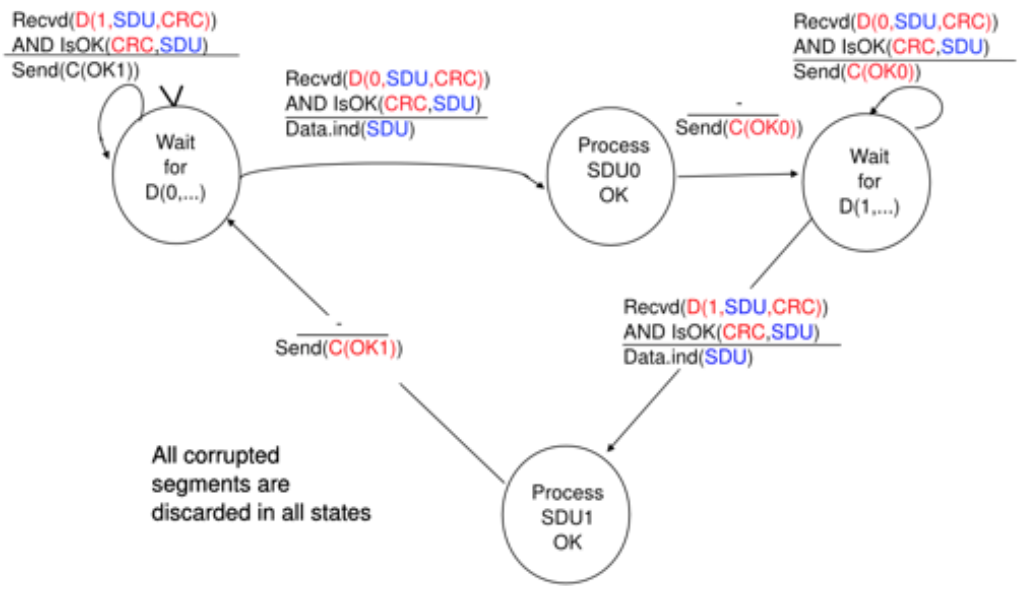
\includegraphics[width=\textwidth]{abp_receiver_fsm.png}
		\caption{\textsc{ABP} receiver \textsc{FSM}.
		The receiver first waits for \texttt{D(0,\dots)}.
		If the frame contains a correct \textsc{CRC},
		it passes the \textsc{SDU} to its user and sends \texttt{OK0}.
		If the \textsc{CRC} is invalid,
		the frame is discarded.
		The receiver then waits for \texttt{D(1,\dots)}.
		In this state,
		it may receive a duplicate \texttt{D(0,\dots)}
		or a data frame with an invalid \textsc{CRC}.
		In both cases, it returns an \texttt{OK0} frame
		to allow the sender to recover
		from the possible loss of the previous \texttt{OK0} frame.}
		\label{fig:abp_receiver_fsm}
	\end{subfigure}
	\caption{\textsc{FSM}s for the \textsc{ABP}.}
	\label{fig:abp_fsm}
\end{figure}

\textsc{ABP} can recover
from transmission errors and frame losses (shown in \figuref{abp_errors}).
However, it has an important drawback:
it has low maximum throughput.

\begin{figure}[H]
	\centering
	\begin{subfigure}[t]{0.31\linewidth}
		\centering
		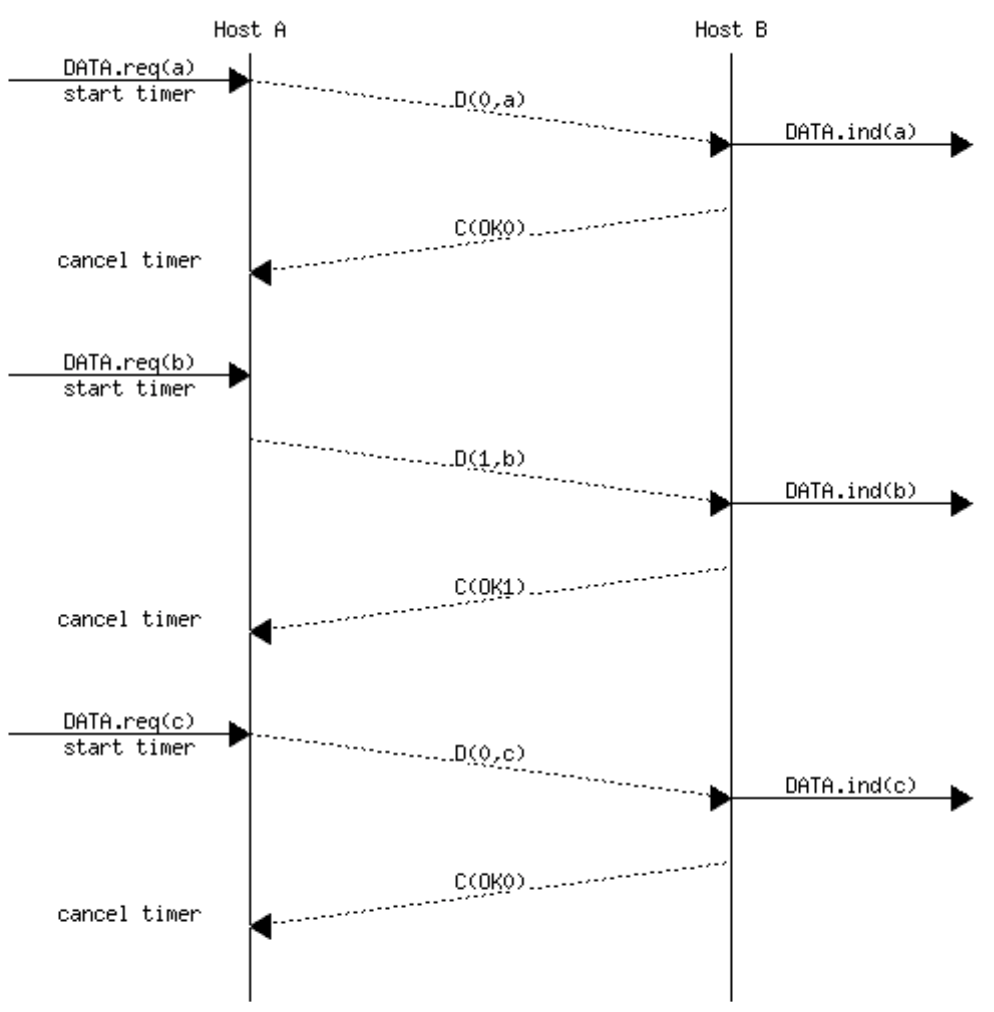
\includegraphics[width=\textwidth]{abp_success.png}
		\caption{A successful transmission with \textsc{ABP}.}
		\label{fig:abp_success}
	\end{subfigure}
	\hfill
	\begin{subfigure}[t]{0.31\linewidth}
		\centering
		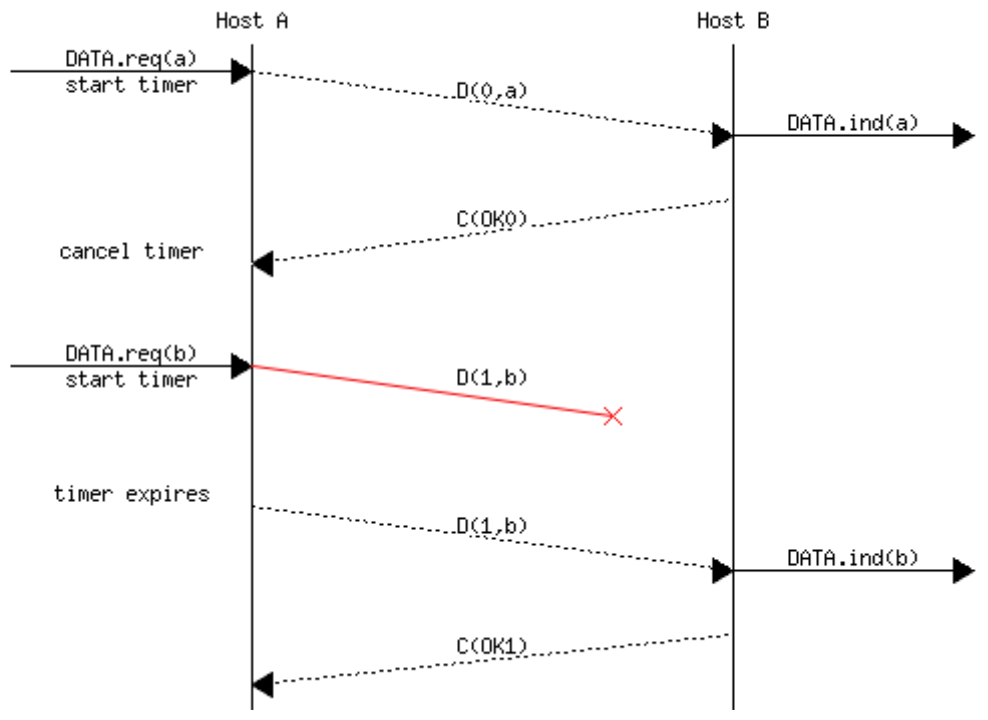
\includegraphics[width=\textwidth]{abp_error_trans.png}
		\caption{\textsc{ABP} can recover from the loss of data frames.}
		\label{fig:abp_error_trans}
	\end{subfigure}
	\hfill
	\begin{subfigure}[t]{0.31\linewidth}
		\centering
		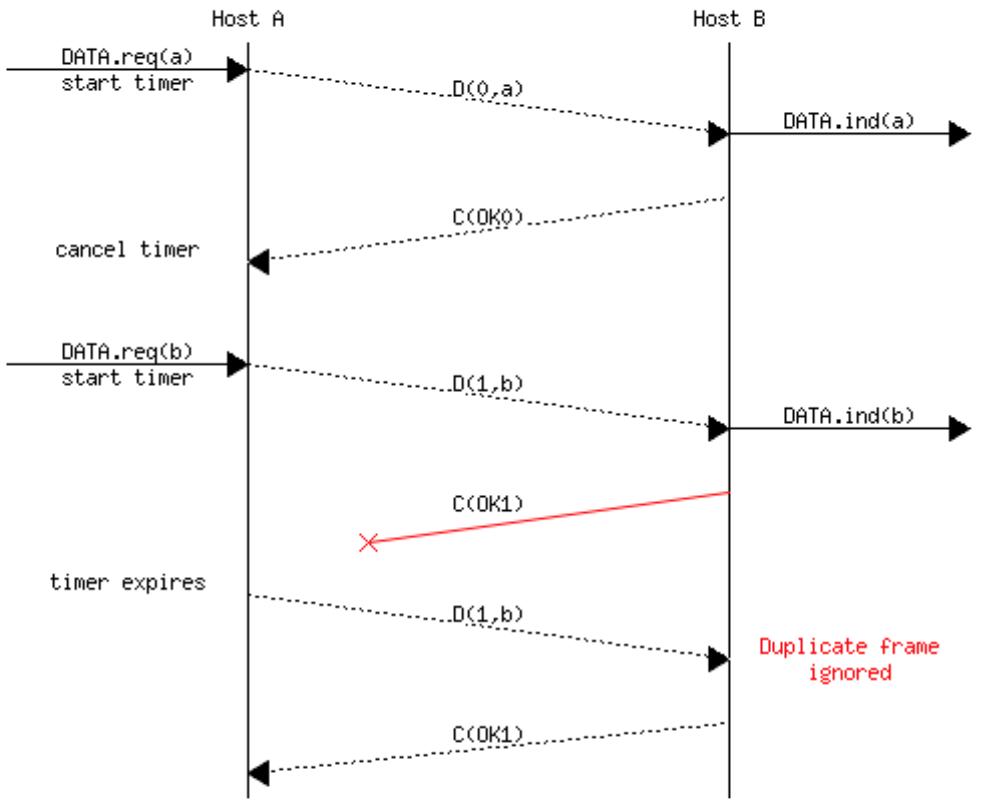
\includegraphics[width=\textwidth]{abp_error_ack.png}
		\caption{\textsc{ABP} can recover
		from the loss of control frames.}
		\label{fig:abp_error_ack}
	\end{subfigure}
	\caption{\textsc{ABP} can recover
	from the losses of data or control frames.}
	\label{fig:abp_errors}
\end{figure}
\subsubsection{Go Back $N$}
To deal with the performance limitations of \textsc{ABP},
reliable protocols rely on \emph{pipelining}.
This means a sender can send multiple consecutive frames
without having to wait for an acknowledgment after each frame.
Each frame contains a seqnum encoded in an $n$-bit field.
Pipelining can possibly overload the receiver,
which is why reliable protocols only allow
$W$ unacknowledged frames to be transmitted
before being forced to wait for an acknowledgment.
This is implemented by using a \emph{sliding window},
like the ones shown in \figuref{sliding_window}.

\begin{figure}[H]
	\centering
	\begin{subfigure}[t]{0.45\linewidth}
		\centering
		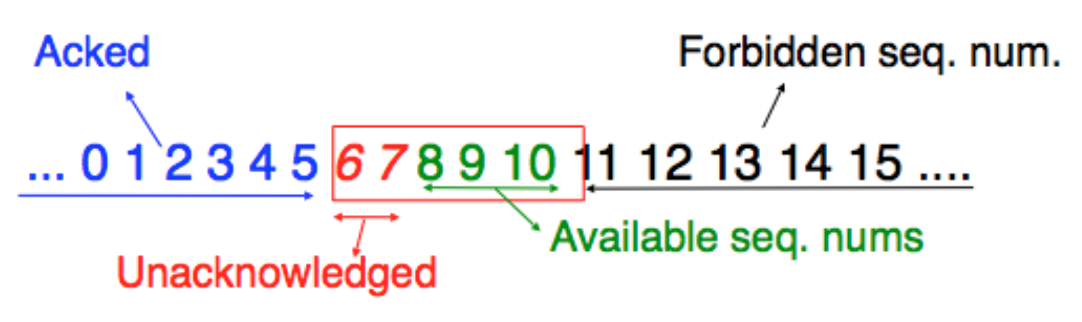
\includegraphics[width=\textwidth]{sliding_window1.png}
		\caption{An example sliding window containing $5$ segments.}
		\label{fig:sliding_window1}
	\end{subfigure}
	\hfill
	\begin{subfigure}[t]{0.45\linewidth}
		\centering
		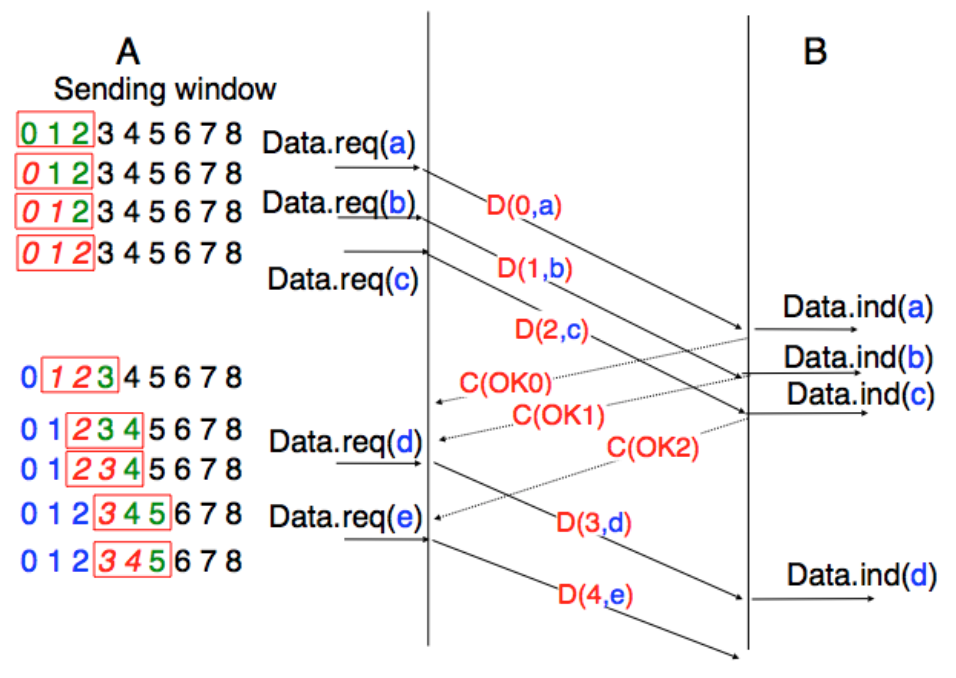
\includegraphics[width=\textwidth]{sliding_window2.png}
		\caption{An example of a sliding window of size $3$
		being used by the sender.}
		\label{fig:sliding_window2}
	\end{subfigure}
	\caption{The sliding window.}
	\label{fig:sliding_window}
\end{figure}

Note that since the headers use an $n$-bit field to encode the seqnum,
only the numbers in the interval $0$--$2^n - 1$ can be used.
This means the sliding window needs to be able to wrap.

To recover from losses,
a sliding window protocol must define
\begin{itemize}
	\item a \emph{heuristic} to detect frame losses and
	\item a \emph{retransmission strategy} to retransmit the lost frames.
\end{itemize}
The simplest such strategy is called Go Back $N$.
It works as follows:
when a receiver receives a frame,
it returns an acknowledgment containing the seqnum of
the last in-sequence frame it received.
This acknowledgment is said to be \emph{cumulative}.
This means that if the frame with seqnum $x$ is acknowledged,
then the sender knows that all previous frames were also received succesfully,
even if their acknowledgments were lost in transmission.
A sender stores a buffer of the size of the sliding window.
The frames are sent with increasing seqnums
($\mod \texttt{maxseq}$).\footnote{\texttt{maxseq} is the maximum number of different sequence numbers ($2^n$).}
Once the sending buffer is full,
it must wait for an acknowledgment.
When the sender receives an acknowledgment,
it removes all the acknowledged frames from the sending buffer,
and uses a retransmission timer to detect frame losses.
This timer is started when the first frame is sent,
and after receicing an acknowledgment,
it only restarts the timer if
there are still unacknowledged frames in the sending buffer.
When the timer expires,
all frames in the buffer are retransmitted
(and the timer is restarted again, etc.).
These possible states are summarized in \figuref{gbn_fsms}.

\begin{figure}[H]
	\centering
	\begin{subfigure}[t]{0.45\linewidth}
		\centering
		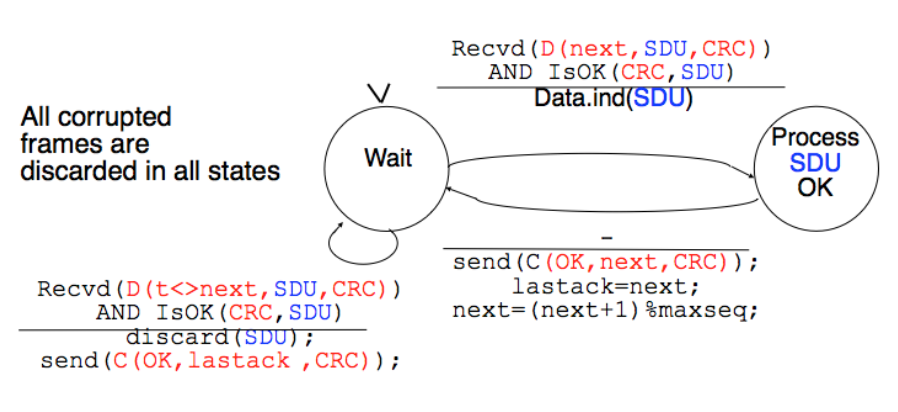
\includegraphics[width=\textwidth]{gbn_receiver_fsm.png}
		\caption{The finite state machine for a Go Back $N$ receiver.
		This receiver uses two variables:
		\texttt{lastack} and \texttt{next}.
		\texttt{next} is the next expected sequence number
		and \texttt{lastack} the sequence number
		of the last data frame that has been acknowledged.
		The receiver only accepts the frames
		that are received in sequence.}
		\label{fig:gbn_receiver_fsm}
	\end{subfigure}
	\hfill
	\begin{subfigure}[t]{0.45\linewidth}
		\centering
		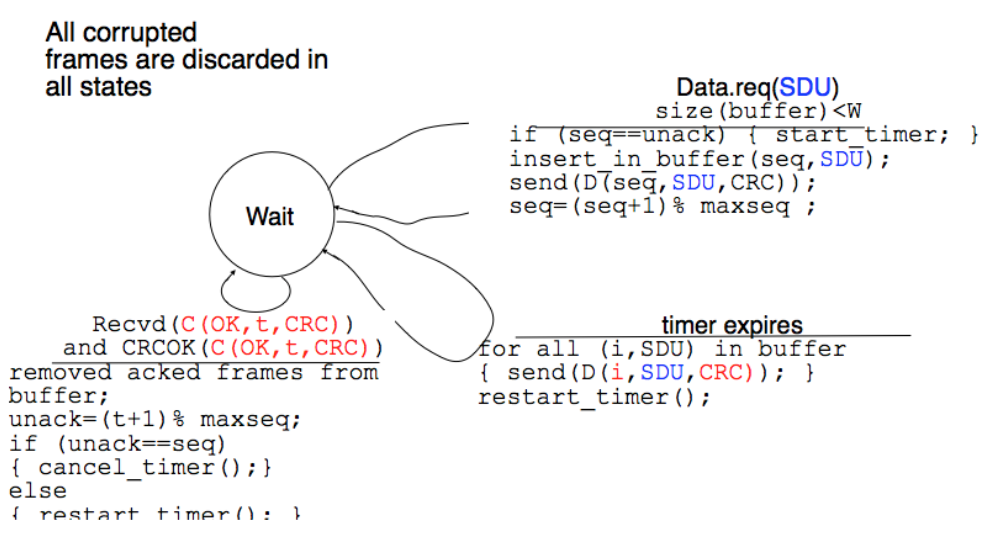
\includegraphics[width=\textwidth]{gbn_sender_fsm.png}
		\caption{The finite state machine for a Go Back $N$ sender.}
		\label{fig:gbn_sender_fsm}
	\end{subfigure}
	\caption{Finite state machines for the Go Back $N$ recovery protocol.}
	\label{fig:gbn_fsms}
\end{figure}

The operation of this protocol is illustrated in \figuref{gbn_ex}.
\begin{figure}[H]
	\centering
	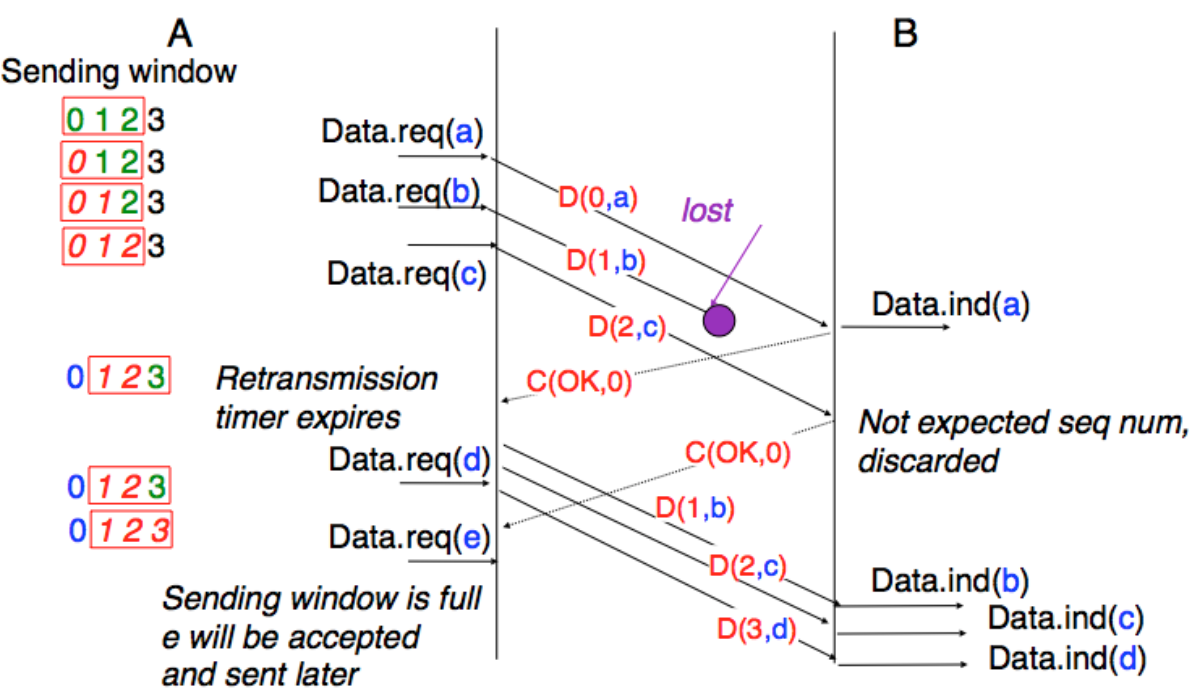
\includegraphics[width=0.6\textwidth]{gbn_ex.png}
	\caption{An example of Go Back $N$ at work.}
	\label{fig:gbn_ex}
\end{figure}

While it is easy to implement,
Go Bac $N$ also has some drawbacks:
when many frames are lost,
performance drops because out-of-sequence frames
are not accepted by the receiver and
the sender retransmits \emph{all} frames once it detects a loss.
\subsubsection{Selective Repeat}
For these reasons,
selective repeat is a smarter strategy.
It has a sliding window of $W$ frames,
just like Go Back $N$,
but it also stores received out-of-frequence frames.
The selective repeat receiver discards all frames with an invalid \textsc{CRC}.
\texttt{lastack} is the last in-sequence frame received,
and it is always included in the acknowledgments that the receiver sends.
Some protocols also allow the selective repeat receiver
to acknowledge the out-of sequence frames that it has received.
This can be done by placing the list of the correctly received,
but out-of-sequence frames together with the \texttt{lastack} value.
When the receiver receives a data frame,
it first verifies whether the frame is inside its receiving window.
If yes, the frame is placed in the receive buffer.
If not, the frame is discarded and an acknowledgment with \texttt{lastack}
is sent to the sender.
The receiver then removes all consecutive frames
starting at \texttt{lastack} (if any) from the receive buffer.
The payloads of these frames are delivered to the user,
\texttt{lastack} and the receiving window are updated,
and an acknowledgment acknowledging the last frame received in sequence is sent.
\bigbreak
The selective repeat sender maintains a sending buffer
that can store up to $W$ unacknowledged frames.
These frames are sent as long as the sending buffer is not full.
Several implementations of a selective repeat sender are possible.
A simple implementation associates one retransmission timer to each frame.
The timer is started when the frame is sent
and cancelled upon reception of an acknowledgment that covers this frame.
When a retransmission timer expires,
the corresponding frame is retransmitted
and this retransmission timer is restarted.
When an acknowledgment is received,
all the frames that are covered by this acknowledgment
are removed from the sending buffer and the sliding window is updated.

\begin{figure}[H]
	\centering
	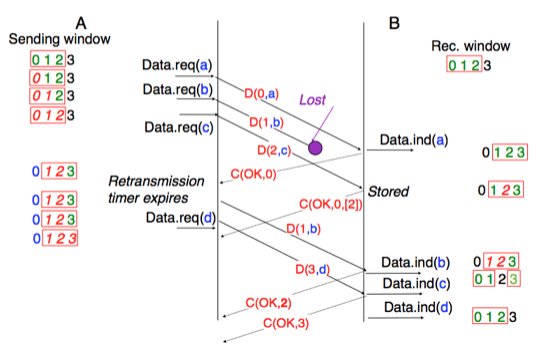
\includegraphics[width=0.6\textwidth]{selective_repeat_ex.png}
	\caption{An example of selective repeat at work.
	The figure illustrates the operation of selective repeat
	when frames are lost.
	In this figure, \texttt{C(OK,x)} is used to indicate that all frames,
	up to and including sequence number $x$ have been received correctly.
	This figure also shows selective acknowledgment,
	which the receiver telling the sender
	about correctly received,
	but out-of-sequence frames.
	The sender knows it should stop the retransmission timers
	for those frames,
	while still keeping them in the sending buffer
	until the reception of a cumulative acknowledgment.}
	\label{fig:selective_repeat_ex}
\end{figure}

\begin{myrem}[Maximum window size with Go Back $N$ and selective repeat]
	Theoretically, the maximum window size for a reliable protocol
	using $n$ bits to encode its seqnums is $2^n$.
	However, consider Go Back $N$ and that all acknowledgments are lost,
	despite the frames being received in-sequence.
	The sender will have to send all the frames again,
	and the user will receive them a second time,
	thinking they're the next batch of frames.
	This can be fixed by using $2^n-1$ instead.
	Something similar happens with selective repeat.
	To avoid this problem and have reliable delivery,
	selective repeat senders should use window of size at most $2^{n-1}$,
	so that the same frame doesn't get accepted multiple times.
\end{myrem}

Reliable protocols often need to send data in both directions.
\emph{Piggybacking} is used to avoid overhead caused by acknowledgments
by allowing the acknowledgments to be sent together with other information.
This only works when data flows in both directions.
If no data is to be sent,
the receiver will simply send a pure acknowledgment (\figuref{piggybacking}).
\begin{figure}[H]
	\centering
	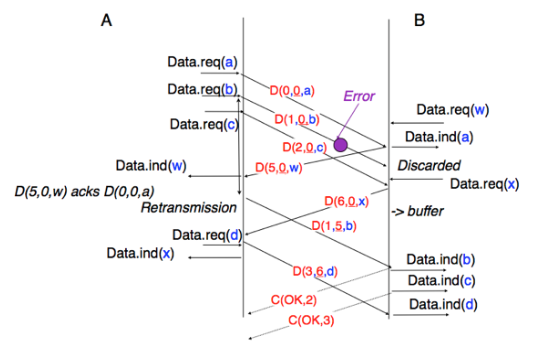
\includegraphics[width=0.6\textwidth]{piggybacking.png}
	\caption{An example of piggybacking being used.
	The bottom of the figure shows
	the receiver sending a pure acknowledgment
	when no data is to be sent in the opposite direction.}
	\label{fig:piggybacking}
\end{figure}

\section{Building a Network}
When hosts aren't connected to each other by a direct physical layer link,
we need to add another layer on top of the datalink layer:
the network layer.

Its main objective is to allow end systems,
connected to different networks,
to exchange information through intermediate systems called routers.
Information is sent in packets in the network layer.

Datalink layers can be either reliable
(if the physical layer is prone to suffer from transmission errors)
or unreliable (if transmission errors are rare).
We assume here that the datalink layer service
provides an \emph{almost reliable} service.

There are two main types of datalink layers:
\begin{itemize}
	\item \emph{Point-to-point} datalink layers are used
	when there are only two communicating systems
	that are directly connected through the physical layer.
	Depending on how high the bit error ratio in the physical layer is,
	the datalink layer will be either reliable or unreliable.
	Point-to-point datalink layers can
	either connect two end systems or two routers.
	\item \textsc{LAN}s\footnote{Local area network} use
	a second type of datalink layer.
	A \textsc{LAN} is a set of communicating devices
	such that any two devices
	can directly exchange frames through the datalink layer.
\end{itemize}

Each datalink layer is characterized by a maximum frame size.
The heterogeneity in the maximum frame sizes can cause problems
when we need to exchange data between hosts
attached to different types of datalink layers.

An example network is represented in \figuref{typ_network}.
\begin{figure}[H]
	\centering
	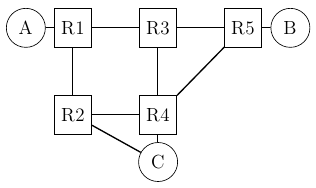
\includegraphics[width=0.4\textwidth]{typ_network.png}
	\caption{A typical network consisting of
	three end systems (or hosts, represented with circles)
	and five routers (represented with boxes).}
	\label{fig:typ_network}
\end{figure}

\begin{mydef}[End system]
	\emph{End systems}, or \emph{hosts},
	are devices which are able to send and receive data for their own usage.
	They are usually attached to the network via a single link.
	A host is \emph{multihomed} if it is equipped
	with several physical interfaces.
\end{mydef}
\begin{mydef}[Router]
	\emph{Routers}, in contrast with hosts,
	usually forward data towards its final destination.
	A router has multiple neighboring routers or hosts.
\end{mydef}

Let's analyze the operations that need to be performed to allow host $A$
in the above network to send one byte to host $B$.
Host $A$ can easily send a frame to router $R_1$ over the datalink layer.
The network layer serves to let $R_1$ know
that the data is for host $B$ and not for the router itself.

The network layer sends packets from host to host,
with intermediate routers in between.
Packets contain the information to be transmitted
as well as control information.
Each node in the network has an address
(usually a sequence of bits of fixed length).

The packet that host $A$ sends to host $B$
either contains the addresses of the source and the destination nodes,
or information that indicates the path that needs to be followed
to reach the destination.

There are two possible organisations for the network layer:
\begin{itemize}
	\item the \emph{datagram organisation} and
	\item \emph{virtual circuits}.
\end{itemize}

\subsection{The Datagram Organisation}
Each host is identified by its \emph{network layer address}.
Hosts create packets containing
\begin{itemize}
	\item the network layer address of the destination host;
	\item its own network layer address;
	\item the information to be sent.
\end{itemize}

Routers in the datagram organisation use \emph{hop-by-hop} forwarding.
Hence, when a router receives a packet that is not destined to itself,
it looks up the destination address in its \emph{forwarding table}.
\begin{mydef}[Forwarding table]
	A forwarding table is a data structure
	that maps each destination address
	with the outgoing interface over which this address must be forwarded.
\end{mydef}

Computing forwarding tables can be done in multiple ways,
but care must be taken so as to make sure that:
\begin{itemize}
	\item No \emph{black holes} occur.
	A black hole is when a router receives a packet with a destination
	for which it does not have an entry in its forwarding table.
	\item Packets do not get caught in an infinite loop.
\end{itemize}

The forwarding table and the format of the packets
are part of the \emph{data plane} of the network.
This data plane contains all the protocols and algorithms
that are used by hosts and routers
to create and process the packets that contain user data.
A network is also characterized by its control plane,
which contains the the protocols and algorithms
used to compute the forwarding tables.
Forwarding tables must be adapted in case of link or router failure.

\subsubsection{Computing Forwarding Tables}
We present three techniques for computing forwarding tables
upon the arrival of a packet.

The first technique assumes that the network topology is a tree.
This means there cannot be cycles or infinite loops.
In this technique,
routers maintain data structures called
\emph{port-address tables},
which map outgoing interfaces to destination addresses.
When the router receives a packet on a certain interface,
it learns that the source host is reachable over that interface,
and adds this to its port-address table.
If the destination address is in the router's port-address table,
it simply forwards the packet on the corresponding interface.
If not,
the packet is \emph{broadcast} over the network
(forwarded over all interfaces except the one it was received over).

This technique has two main drawbacks:
\begin{itemize}
	\item If the destination is not in the network,
	the packet gets broadcast repeatedly.
	\item Few networks have the required tree-shaped topology.
	If the network does not have this topology,
	packets can get caught in infinite loops easily.
\end{itemize}

Another technique, called \emph{source routing},
enables a destination to discover the paths
from a given source to itself,
by relying on network nodes to change some information inside packets.
We assume the data plane supports two types of packets:
data packets and control packets.

Data packets are used to exchange data,
while control packets are used to discover paths between endhosts.
When a host or router starts,
it sends a special control packet over all of its interfaces
to advertise its address to its neighbors.
When a host or node receives this control packet,
it replies with its own address.
This can also allows checking whether a neighbor is still alive.
With source routing, the data plane packets include a list of identifiers,
called a \emph{source route}.
This list is the path to be followed by the packet.
When a router receives such a packet, it forwards the packet
over the next interface in the sequence of identifiers.

Control packets contain a list that records the intermediate nodes.
When a router receives a control packet,
it looks for its own address in this \emph{record route}.
If it is included, the packet is discarded,
if not, the node adds its own address to the record route
and broadcasts the packet.
When a host receives multiple copies of the same packet,
the one that arrived first is supposed to have the best route.

Once the destination host receives the packet,
it can simply reverse the record route
and send a data packet to let the source node know the route.

\subsubsection{Flat Or Hierarchical Addresses}
There are two ways in which addresses can be organized.
Addresses are encoded as bit strings.

Under the flat addresssing scheme,
each host and network node has a unique address.
With this scheme,
the lookup operation in the forwarding table can be implemented
with binary search if the list of addresses is sorted,
hence it has complexity $\bigoh(\lg n)$.

However, a drawback of this scheme is that
the size of the forwarding tables grows
linearly with the number of hosts and nodes in the network.

The second scheme is called hierarchical addressing,
and it divides the address into parts,
where each part narrows down the number of possible addresses.
The addressing space is divided in consecutive blocks,
then these blocks are allocated to different parts of the network.

The main advantage of hierarchical addressing over flat addressing
is the significantly reduced forwarding table size.
The drawbacks are
\begin{itemize}
	\item lookup operations become more complicated,
	\item when a host first connects to a network,
	it must contact a node to determine its own address and
	\item if a host moves, its address can change.
\end{itemize}

\subsubsection{Dealing With Heterogeneous Datalink Layers}
When a network needs to deal with heterogeneous datalink layers,
exchanging packets becomes possible thanks to the network layer,
provided that the packet can be placed inside a datalink layer frame
before being transmitted.

If a router finds a packet that is too large
to be forwarded inside a single frame,
multiple solutions exist:
\begin{itemize}
	\item the router can send the packet back to the source host
	indicating it cannot forward packets
	longer than a certain amount of bytes;
	\item the network layer fragments the packets in two fragments
	before transmitting them,
	and then they are reassembled by the next router;
	\item the fragments are valid packets,
	and are treated as regular packets by the next routers,
	meaning the destination host receives them as two separate packets.
\end{itemize}

The first solution is simple
and does not require routers to do any fragmentation.
Hosts are more complex however,
because they need to store the packets they produce
if they pass through a narrow link.

Fragmenting the packets on a per-link basis
can minimize the transmission overhead.
Two drawbacks are that processing time
and buffer requirements on the routers are increased.
It also leads to a longer end-to-end delay since the downstream router
has to reassemble the fragments before forwarding the original packet.

The last solution is a compromise between the two others.
It has a lowed end-to-end delay
and requires less processing time and memory on the routers.

The first solution suggests using control packets
to inform the source about the reception of a long packet.
This is one of the functions of the control protocol; the others are
\begin{itemize}
	\item sending a control packet to the source
	if a router does not have a valid entry in its forwarding table;
	\item sending a control packet
	when a looping packet is detected inside the network;
	\item verifying that packets can reach a given destination.
\end{itemize}

\subsection{Virtual Circuit Organisation}
In a network using virtual circuits,
all hosts are identified with a network layer address.
Each packet contains a \emph{label} in its header,
which can be switched by routers.
When it receives a packet,
the router looks for this packet in its \emph{label forwarding table}
to find which interface the packet must be forwarded over.
The lookup operation has constant complexity as the table is stored as an array.
The table also indicates what the label of the outgoing packet should be set to.
The label forwarding table contains two pieces of information:
\begin{itemize}
	\item the outgoing interface for the packet;
	\item the label for the outgoing packet.
\end{itemize}
Label switching allows users to have full control
over the path followed by the packets inside the network.

Multi-Protocol Label Switching (\textsc{mpls})
is a deployed networking technology that relies on label switching.
It is more complicated than the above description however.
The control plane contains distributed algorithms,
called \emph{routing protocols},
to compute the forwarding tables that are installed on the network nodes.
Two main families of routing protocols exist:
\emph{distance vector routing} and \emph{link state routing}.

\subsection{The Control Plane}
One of the objectives of the control plane in the network layer
is to maintain the routing tables.

\subsubsection{Distance Vector Routing}
With distance vector routing,
the shortest path between hosts is computed based on \emph{metrics}
that are associated to each link.
We used \texttt{l.cost} to represent the metric
that has been configured for link \texttt{l} on a router.

Each router maintains a routing table.
The routing table \texttt{R} can be modelled as a data structure
that stores, for each known destination address \texttt{d},
the following attributes:
\begin{itemize}
	\item \texttt{R[d].link} is the outgoing link
	used to forward packets to \texttt{d};
	\item \texttt{R[d].cost} is the sum of the metrics of the links
	that compose the shortest path to reach \texttt{d};
	\item \texttt{R[d].time} is the timestamp
	of the last distance vector containing destination \texttt{d}.
\end{itemize}

A router using distance vector routing regularly sends its distance vector
over all its interfaces.
The distance vector is a summary of the router's routing table
that indicates the distance towards each known destination.

When a router receives a distance vector on link \texttt{l},
it iterates over all addresses in the distance vector.
It updates its routing table as follows:
\begin{itemize}
	\item If the distance vector contains a previously unknown address,
	the destination is inserted inside the routing table via link \texttt{l}
	and at a distance which is the sum between
	the distance in the vector and the cost of link \texttt{l}.
	\item If the address was previously known,
	the entry is updated if
	\begin{itemize}
		\item the cost of the new route is smaller than the one
		in the table (if \texttt{V[d].cost + l.cost < R[d].cost});
		\item the new route was learned over the same link
		as the current best route (\texttt{R[d].link = l}).
	\end{itemize}
	The first condition ensures that the router
	discovers the shortest path to each destination,
	while the second is used to take into account
	changes of routes in case something in the network changes.
\end{itemize}

To deal with link and router failures,
routers use the timestamp in their routing table.
Routers send their distance vector every $N$ seconds,
thus no route should have a timestamp older than $N$ seconds,
unless it is not reachable anymore.
In practice, the cutoff is at $3N$ seconds:
all routes that are older than this value
are removed when the router checks its table's timestamps every $N$ seconds.
When a router notices a route towards a destination has expired,
it associates an infinite cost to this route
and sends a distance vector to neighboring routers to inform them.
After some more waiting (typically $3N$ seconds),
the entry can be removed from the routing table.

In some situations, a problem known as ``\emph{count to infinity}'' can occur,
when two routers exchange distance vectors with increasing costs.
This problem can appear as soon as the network contains cycles.
Some protocols consider that $16$ is infinity
to mitigate the impact of counting to infinity.
This limits the metrics that operators can use
and the diameter of networks using distance vectors.

The problem occurs when a router $R_1$ advertises to another router $R_2$
a route that it has learned via $R_2$.
A solution is then a technique called \emph{split-horizon},
where routers create distance vectors that are specific to each neighbor
and only contain routes that have not been learned via this neighbor.
Another variant called \emph{split-horizon with poison-reverse}
is used as well.
In this case, routers advertise an infinite cost
for destinations that they reach
via the router to which they send the distance vector.
Not all count to infinity problems can be avoided with these techniques however.

\begin{myrem}[Forwarding tables versus routing tables]
	Routers usually maintain both a \emph{routing table}
	and a \emph{forwarding table}.
	The routing table associates a destination to an outgoing interface
	or a nexthop router, and a set of additional attributes.
	Different routing protocols store different attributes.
	Distance vector routing protocols
	will store the cost to reach the destination along the shortest path.
	The routing table is usually not directly used when forwarding packets,
	as this operation relies on a more compact data structure
	called a \emph{forwarding table}.
	This forwarding table contains
	a subset of the information found in the routing table.
	It only contains the paths that are used to forward packets,
	associating each destination to an outgoing interface or nexthop router.
\end{myrem}

\subsubsection{Link-State Routing}
Link-state routing is based on routers exchanging messages
to allow each router to learn the entire network topology.

A network is modelled as a \emph{directed weighted graph}.
Each router is a node, the links are the edges in the graph
and the weights are associated according to one of these options:
\begin{itemize}
	\item unit weights;
	\item weight proportional to the propagation delay on the link;
	\item $\textnormal{weight} = \frac{C}{\textnormal{bandwidth}}$,
	where $C$ is a constant greater than the highest bandwidth.
\end{itemize}
Routers use the shortest path to reach each destination.

When a link-state router first boots,
it sends a \texttt{HELLO} message every $N$ seconds on all of its interfaces.
This message contains the router's address.
This allows all routers to know which other routers they are connected to.
\texttt{HELLO} messages are never forwarded,
and a link is considerd to have failed if
no \texttt{HELLO} message has been received from the neigboring router
for a period of $kN$ seconds.

Once a router has discovered its neighbors,
it builds \emph{link state packets} (\textsc{lsp}s),
to distribute its local links to all routers in the network.
A \textsc{lsp} contains the following information:
\begin{itemize}
	\item \texttt{LSP.router}:
	identification of the sender of the \textsc{lsp}.
	\item \texttt{LSP.age}:
	remaining lifetime of the \textsc{lsp}.
	\item \texttt{LSP.seq}:
	sequence number of the \textsc{lsp}.
	\item \texttt{LSP.links[]}:
	links advertised in the \textsc{lsp}.
	Each directed link contains the following information:
	\begin{itemize}
		\item \texttt{LSP.links[i].id}: identification of the neighbor.
		\item \texttt{LSP.links[i].cost}: cost of the link.
	\end{itemize}
\end{itemize}
The \emph{flooding} algorithm is used to distribute \textsc{lsp}s.
Each router maintains a link-state database (\textsc{lsdb})
containing the most recent \textsc{lsp} sent by each router.
When a router receives a \textsc{lsp},
it verifies whether this packet is already stored in its database.
If not, the packet is broadcast.
If it is in the database, then the packet has already been broadcast before,
and does not need to be broadcast again.

\begin{myrem}[Determining the most recent \textsc{lsp}]
	The comparison should take into account the modulo arithmetic
	used to increment the sequence numbers,
	hence divide the circle of all sequence numbers into two halves.
	Current link-state routing protocols
	use $\SI{32}{\bit}$ sequence numbers
	and include a special mechanism
	in case a sequence number reaches the maximum value.
	\textsc{lsp}s contain a checksum to deal with memory corruption,
	which can cause the algorithm to fail.

	Each router must verify the checksum
	when it receives or floods a \textsc{lsp}.
	Furthermore, each router must periodically verify the checksums
	of the \textsc{lsp}s stored in its \textsc{lsdb}.
\end{myrem}

Flooding allows \textsc{lsp}s to be distributed
to all routers inside the network without relying on routing tables.
To avoid sending the same \textsc{lsp} twice on the same link,
routers wait for a random time before forwarding \textsc{lsp}s.
In practice,
this is only done for ``refresh \textsc{lsp}s'',
as packets with new information are immediately flooded.

Link-state protocols use reliable flooding
to ensure all routers receive all \textsc{lsp}s.
To achieve this,
routers use acknowledgments and, if necessary, retransmissions.

When a link fails,
the two routers attached to this link generate and flood new \textsc{lsp}s
that no longer contain the failed link.
This might not happen at exactly the same time,
hence when other routers receive the \textsc{lsp}
of only one of the attached routers,
they still consider the link as having failed,
and remove it from the directed graph
that they compute from their \textsc{lsdb}.
When a link comes up, it can only be used
once both attached routers have advertised it in their \textsc{lsp}s.
This \emph{two-way connectivity check} also ensures that
failed routers are removed from the graph.

When a router has failed, it must be removed from the databases of all routers.
This can be done by decreasing the \texttt{age} field in each \textsc{lsp}.
Routers regularly decrement the age of the \textsc{lsp}s in their database,
and discard them once they reach zero.

To compute its forwarding table, each router computes the spanning tree
rooted at itself using Dijkstra's shortest path algorithm.
The forwarding table can be derived automatically from the spanning tree.

\section{The Transport Layer}
The \emph{network layer} ensures the delivery of packets on a hop-to-hop basis
through intermediate nodes.
It provides a service to the upper layer called the \emph{transport layer},
that improves the service provided by the network layer
to make it usable by applications.

Most networks use a datagram organisation and provide a simple service
which is called the \emph{connectionless service}.
The connectionless service is represented as follows on a time-sequence diagram:
a source with address \texttt{S} issues
a \texttt{Data.request} primitive (\texttt{Data.request(S, D, `M')})
containing a Service Data Unit (\textsc{sdu}) \texttt{M}
that must be delivered to destination \texttt{D},
which delivers the corresponding
\texttt{Data.indication} primitive
to the user (\texttt{Data.indication(S, D, `M')}).

A \emph{reliable connectionless service} is a service
where the service provider guarantees that all \textsc{sdu}s
submitted in \texttt{Data.request}s by a user
will eventually be delivered to their destination.
In practice, an \emph{unreliable connectionless service} is often supported.
As the transport layer is built on top of the network layer,
it is important to know the key features
of the \emph{(connectionless) network layer service}:
\begin{itemize}
	\item it can only transfer \textsc{sdu}s of \emph{limited size};
	\item it may discard \textsc{sdu}s;
	\item it may corrupt \textsc{sdu}s;
	\item it may delay, reorder of even duplicate \textsc{sdu}s.
\end{itemize}
The main cause of packet losses and errors
are the buffers used on the network nodes.

\subsection{Transport Layer Services}
When two applications need to communicate,
they need to structure their exchange of information.
This requires solving two problems:
\begin{itemize}
	\item How to represent information being exchanged.
	\item How to organise the interactions
	between the application and the underlying network.
	From the application's viewpoint,
	the network will appear as the \emph{transport layer service}.
	This layer provides three types of services to the applications:
	\begin{itemize}
		\item the \emph{connectionless service};
		\item the \emph{connection-oriented service};
		\item the \emph{request-response service}.
	\end{itemize}
\end{itemize}

\subsubsection{The Connectionless Service}
The \emph{connectionless service} is used to exchange small \textsc{sdu}s.
It can easily be built on top of the connectionless network layer service
described earlier.

\subsubsection{The Connection-Oriented Service}
This service is used when users need to send or receive
several different and potentially large \textsc{sdu}s,
or by users who need structured exchanges.
An invocation of the \emph{connection-oriented service}
is divided into three phases:
\begin{enumerate}
	\item Establishment of a \emph{connection}.
	\begin{mydef}[Connection]
		A \emph{connection} is a temporary association
		between two users through a service provider.
		Several connections may exist at the same time
		between any pair of users.
		Connections are used to transfer \textsc{sdu}s,
		and they usually provide one bidirectional stream
		supporting the exchange of \textsc{sdu}s.
	\end{mydef}
	\item \emph{Data transfer phase}.
	The stream provided by the connection is used to transfer data.
	\item \emph{Termination} of the connection.
	Once users are done exchanging \textsc{sdu}s,
	they request termination of the connection from the provider.
\end{enumerate}

\paragraph{Connection Establishment}
The establishment of a connection can be modelled using four primitives:
\begin{itemize}
	\item \texttt{Connect.request}, used to request the connection;
	\item \texttt{Connect.indication}, delivered by the provider
	to inform the destination user of the connection attempt;
	\item \texttt{Connect.response}, sent if the destination user
	accepts the connection;
	\item \texttt{Connect.confirm}, delivered by the provider
	to the user who initiated the connection.
\end{itemize}
The destination user can start sending \textsc{sdu}s
after sending a \texttt{Connect.response}.
The connection is open after sending the \texttt{Connect.confirm} primitive,
and both users can send \textsc{sdu}s at that point.

Two reasons for why a connection might fail to be established are:
\begin{itemize}
	\item The destination user may not agree to establish a connection,
	and responds to the \texttt{Connect.indication}
	with a \texttt{Disconnect.request}.
	The provider then delivers a \texttt{Disconnect.indication}
	to the initiating user.
	\item If the provider is unable to reach the destination,
	it responds to the \texttt{Connect.request}
	with a \texttt{Disconnect.indication}.
\end{itemize}

\paragraph{Data Transfer Phase}
Two streams are supplied to the communicating users:
\begin{itemize}
	\item the first can be used by the initiator to send \textsc{sdu}s;
	\item the second allows the responding user to send \textsc{sdu}s.
\end{itemize}

These streams can be organised in different ways:
\begin{itemize}
	\item \emph{Message-mode transfer}.
	With this organisation,
	the service prodiver guarantees that only one \texttt{Data.indication}
	will be delivered for each \texttt{Data.request}.
	\item \emph{Stream-mode transfer}.
	The service provider supplies a byte stream
	that links the two communicating users.
	\textsc{sdu}s are sent as sequences of bytes.
	The provider guarantees the order in which the bytes arrive is correct,
	but does not attempt to preserve the boundaries of the \textsc{sdu}s.
	No relation is enforced between
	the number of \texttt{Data.request}
	and \texttt{Data.indication} primitives.
	Users have to provide the mechanisms that allow the receiving user
	to separate successive \textsc{sdu}s
	in the byte stream that it receives.
\end{itemize}

\paragraph{Connection Release}
Connections involve three parties (two users and a provider),
and each one of them can request connection termination.
Two types of connection release exist:
\begin{itemize}
	\item \emph{Abrupt connection release}.
	This type of release can be triggered by the provider and the users,
	and can cause losses of data.
	If the provider requests it,
	it sends a \texttt{Disconnect.indication} primitive
	to both users.
	When a user requests it,
	the user sends a \texttt{Disconnect.request(abrupt)} primitive
	to the provider, which then stops the two data streams
	and delivers the \texttt{Disconnect.indication} primitive
	to the remote user.
	\item \emph{Graceful connection release}.
	We consider both streams to be independent.
	One user issues a \texttt{Disconnect.request(graceful)} primitive
	to their provider after sending their last \texttt{Data.request},
	then closes their outbound communications.
	The provider sends all \texttt{Data.indication} primitives,
	then send the \texttt{Disconnect.indication}.
	This tells the other user that they will no longer receive \textsc{sdu}s
	over this connection,
	but are still able to issue \texttt{Data.request} primitives
	on the stream in the opposite direction,
	hence this user can close their inbound communications.

	When the user is done issuing \texttt{Data.request} primitives,
	they send a \texttt{Disconnect.request(graceful)} primitive
	to the provider,
	and close their outbound communications.
	The provider issues the necessary \texttt{Data.indication} primitives,
	then follows up with a \texttt{Disconnect.indication}.
	The other user receives this primitive
	and closes their inbound communications,
	The two streams have been released successfully,
	and the connection is completely closed.
\end{itemize}

\begin{myrem}[Reliability of the connection-oriented service]
	The connection-oriented service can only guarantee correct delivery
	of all \textsc{sdu}s
	provided that the connection has been released gracefully.
	While the connection is active, there is no such guarantee,
	as the connection may be released abruptly at any time.
\end{myrem}

\subsubsection{The Request-Response Service}
The \emph{request-response service} is a compromise
between the connectionless service and the connection-oriented service.
It allows to efficiently exchange small amounts of information in a request
and associate it with the corresponding response.

\subsection{The Transport Layer}
The transport layer entity allows to deal with some issues of the network layer.

\subsubsection{Connectionless Transport}
This transport service includes two additional features
on top of the connectionless network layer service.
\begin{itemize}
	\item an \emph{error detection} mechanism
	that allows to detect corrupted data;
	\item a \emph{multiplexing technique}
	that enables several applications running on one host
	to exchange information with another host.
\end{itemize}

\textsc{sdu}s are encapsulated inside \emph{segments}.
\begin{mydef}[Segment]
	The \emph{segment} is the basic unit of information
	transferred in the transport layer.
	When the transport layer entity creates a segment,
	it is encapsulated by the network layer
	into a packet with the segment as its payload and a network header.
	The packet is then encapsulated in a frame
	to be transmitted in the datalink layer.
	A segment also contains control information
	stored inside a \emph{header}.
\end{mydef}
Transport protocols rely on
checksums or \textsc{crc}s to detect transmission errors.

In order to differentiate applications running on a host,
the transport layer provides \emph{port numbers}.
Thanks to these port numbers, the transport layer
can allow applications running on one host
to exchange information with another host.

\subsubsection{Connection-Oriented Transport}
To support the connection-oriented service,
the transport service needs to include several mechanisms
to enrich the connectionless network layer service.

\paragraph{Connection Establishment}
The connection-oriented service makes the same use of port numbers
and checksums / \textsc{crc}s as the connectionless service.
An important difference between them however is the fact that
the transport entities in the connection-oriented service
maintain some state during the lifetime of the connection.
This state is created when a connection is established,
and is removed when it is released.

Establishing a transport connection requires
defining two special control segments:
\begin{itemize}
	\item \texttt{CR}, sent by the transport entity
	that wishes to initiate a connection;
	\item \texttt{CA}, used by the remote entity to accept the connection.
\end{itemize}
Both contain port numbers that allow to identify the communicating applications.
The transport connection is said to be ``established''
once the \texttt{CA} segment has been received
(at that point, segments can be sent in both directions).
The control segments must be protected using a checksum / \textsc{crc},
and the \texttt{CR} segment can be protected using a retransmission timer.

Transport protocols also require the network layer
to bound the \emph{Maximum Segment Lifetime} (\textsc{msl}).
Segments must not remain in the network
for longer than $\textnormal{msl}$ seconds (two minutes on the Internet).
To distinguish between duplicate and new \texttt{CR}s,
a \emph{transport clock} with the following characteristics
is used inside each entity:
\begin{itemize}
	\item The clock is implemented as a $k$-bit counter,
	and its clock cycle
	is such that $2^k \times \textnormal{cycle} \gg \textnormal{MSL}$.
	The clock counter is incremented every clock cycle
	and after each connection establishment.
	\item The clock must continue to be incremented
	even if the transport entity stops or reboots.
\end{itemize}

This clock can be combined with an exchange of three segments,
called the \emph{three-way handshake},
to detect duplicates:
\begin{enumerate}
	\item The initiating transport entity sends a \texttt{CR} segment,
	with a port number and a segment number, \texttt{seq = x},
	extracted from the clock.
	The transmission is protected by a retransmission timer.
	\item The remote transport entity processes the \texttt{CR} segment,
	and creates a state for the connection attempt.
	It returns a \texttt{CA} segment
	that acknowledges the reception of the \texttt{CR} segment,
	\texttt{ack = x} and has a sequence number
	extracted from the clock, \texttt{seq = y}.
	\item The initiating entity receives the \texttt{CA} segment.
	The connection is considered to be established by the initiating entity
	and sequence numbers start their numbering at \texttt{x}.
	Before sending data, the initiating entity
	must acknowledge the received \texttt{CA} segments
	by sending another \texttt{CA} segment.
	\item The remote entity considers the transport connection
	to be established after having received the acknowledgment
	for its \texttt{CA} segment.
	Data segment numbering starts at sequence number \texttt{y}.
\end{enumerate}

This three-way handshake avoids duplicate transport connections.
Consider the following three scenarios:
\begin{itemize}
	\item If the remote entity receives an old \texttt{CR} segment,
	it replies with a \texttt{CA} segment.
	The initiating host cannot match this segment
	with a previous connection attempt,
	hence it sends a control segment, \texttt{REJECT},
	to cancel the spurious connection attempt.
	The remote entity cancels the connection attempt
	upon reception of this control segment.
	\item If the initiating entity sends a \texttt{CR} segment
	that does not reach the remote entity,
	and receives a duplicate \texttt{CA} segment
	from a previous connection attempt,
	it finds that the acknowledgment cannot be valid,
	and retransmits the \texttt{CR} segment upon expiration of the timer.
	\item If in the first scenario,
	the control segment fails to be delivered,
	and a duplicate \texttt{CA} segments reaches the remote host instead,
	the remote host realises that the acknowledgment has the wrong number
	hence it sends a control segment (\texttt{REJECT}) of its own.
\end{itemize}

\paragraph{Data Transfer}
The transport protocol must include sliding windows,
retransmission timers and Go Back $N$ or selective repeat,
but cannot simply reuse techniques from the datalink layer.
The differences between the two layers are:
\begin{itemize}
	\item The transport layer must face with more variable delays.
	This happens because packets sent through a network
	do not necessarily follow the same path to their destination.
	Second, some packets may be queued in the buffers of routers,
	which can increase end-to-end delay.
	\item A network does not always deliver packets in sequence.
	\item The network may sometimes duplicate packets.
	\item The transport layer needs to include mechanisms
	to fragment and reassemble large \textsc{sdu}s.
\end{itemize}

However, both layers use checksums / \textsc{crc}s
to detect transmission errors.
Each segment contains one which is computed over the entire segment
(header and payload) by the sender and inserted in the header.
They also use sequence and acknowledgment numbers,
but in the transport layer,
the sequence number in the segment header corresponds to
the position of the first byte of the payload in the bytestream.
This allows to detect losses but also to reorder out-of-sequence segments.
It also makes fragmenting \textsc{sdu}s easier.

Sequence numbers in the transport layer are often longer
than in the datalink layer,
because they must be greater than
the number of bytes transmitted during the \textsc{msl} period.

Most transport protocols use selective repeat instead of Go Back $N$,
as transport entities should always store the segments
that it receives out-of-sequence.

A transport protocol should also allow the sender and the receiver
to adjust their window sizes,
as the memory which can be used to support
the sending or the receiving buffer of a transport connection
may change during the lifetime of the connection.

Transport protocols allow the receiver to advertise
the current size of its receiving window
in all the acknowledgments that it sends.
The sender maintains two state variables:
\begin{itemize}
	\item \texttt{swin}, the size of its sending window;
	\item \texttt{rwin}, the size of the receiving window
	advertised by the receiver.
\end{itemize}
The number of unacknowledged segments cannot be larger
than $\min(\texttt{swin}, \texttt{rwin})$.
To solve deadlock problems that can arise when the receiver advertises
a window of size $0$,
transport protocols rely on a timer called the \emph{persistence timer}.
This timer is started by the sender
whenever a receiving window of $0$ is advertised.
When the timer expires, the sender retransmits and old segment
to force a new acknowledgment.

To deal with ambiguities caused by excessive delays,
transport protocols combine large sequence number fields
with a \emph{Maximum Segment Lifetime}
to ensure segments arriving in the wrong order are handled appropriately.
If a transport protocol uses $n$ bits to encode its sequence numbers,
it cannot send more than $2^n$ segments every $\textnormal{MSL}$ seconds.

\paragraph{Connection Release}
Two methods exist to release a transport connection:
\begin{itemize}
	\item Defining a new control segment (\texttt{DR}),
	and considering the connection to be released
	once this segment has been sent or received.
	This allows abrupt connection releases.
	\item Release the two directions of data transfer independently.
	When a user has sent all of their \textsc{sdu}s,
	they send a \texttt{Disconnect.request}
	for their direction of data transfer.
	The transport entity sends a control segment
	to request connection release after having sent
	all of the remaining \texttt{Data.indication} primitives.
	The remote host confirms the reception of the \texttt{DR} segment
	and the release of the corresponding direction of data transfer
	by returning an acknowledgment.
	Something similar then happens in the other direction
	once the remote host has finished sending \textsc{sdu}s.
	This constitutes a graceful connection release.
\end{itemize}

\section{Sharing Resources}
\subsection{Sharing Bandwidth}
\begin{myrem}[Fairness in computer networks]
	The most widely used definition of \emph{fairness}
	is the \emph{max-min fairness}.
	A bandwidth allocation in a network is said to be \emph{max-min fair}
	if it is such that it is impossible to allocate more bandwidth
	to one of the flows without reducing the bandwidth of a flow
	that already has a smaller allocation than
	the flow that we want to increase.

	If the network is completely known,
	we can find a \emph{max-min fair} allocation
	as follows:
	\begin{enumerate}
		\item initially, all flows have a null bandwidth
		and are placed in the candidate set;
		\item then, we increase the bandwidth allocation
		of all flows in the candidate set
		until one link becomes congested;
		\item the flows using the congested link
		are removed from the candidate set,
		and the process is repeated,
		until the candidate set becomes empty.
	\end{enumerate}
\end{myrem}

\subsection{Network Congestion}
Besides the link bandwidth,
the buffers on the network nodes are the second type of resource
that needs to be shared inside the network.
These buffers are important because they can be used
to absorb transient traffic peaks.
We say that a network is \emph{congested}
when the sum of the traffic demand from the hosts
is larger than the network capacity.
Multiple solutions exist,
but most of the time it is impossible to completely avoid congestion,
and transient congestion is allowed.

The amount of buffering on the network node is the first parameter
that a network operator can tune to control congestion.
Increasing the buffer size on the network nodes
can lead to a problem called ``\emph{congestion control}''.
As two hosts send packets to the same network node,
the buffer on this node fills up,
and sending acknowledgments takes a longer time.
The hosts start retransmitting some of the packets,
amplifying this effect more and more.

A third resource that needs to be shared inside a network
is the packet processing capacity.
In order to forward packets, network nodes need to analyze the packet headers
to perform a lookup inside their forwarding table.
The packet processing rate is mesured in packets per second.

\begin{myrem}[Packets per second versus bits per second]
	The performance of network nodes
	can be characterized by two key metrics:
	\begin{itemize}
		\item the node's capacity measured in bits per second;
		\item the node's lookup performance
		measured in packets per second.
	\end{itemize}

	The capacity depends mainly on the physical interfaces that are used
	and on the capacity of the internal interconnection
	(bus, crossbar switch, \ldots).
	Network nodes should have a capacity
	larger than the sum of their link capacities.
	This maximum is reached when forwarding small packets.

	When a network node forwards small packets,
	its performance is usually limited by
	the number of lookup operations it can perform per second.
	This lookup performance is measured in packets per second.
	The key performance factor is the number of
	minimal size packets that are forwarded by the node every second.
	This rate can lead to a capacity in bits per second which is
	much lower than the sum of the bandwidth of the node's links.
\end{myrem}

In order to adapt their traffic demand
to the current state of the network and the available bandwidth,
hosts need to sense the current level of congestion
and adjust their own traffic demand based on the estimated congestion.
Network nodes can react in different ways to network congestion
and hosts need sense the level of congestion in different ways.

One of the first manifestations of congestion on network nodes
is the saturation of the network links,
which leads to a growth in the occupancy of the buffers of the node,
which in turn leads to longer round-trip times
between the transmission of a packet
and the return of the corresponding acknowledgment.
If hosts measure this round-trip time,
they could sense congestion.
If the buffer's occupancy continues to grow,
the buffer will overflow and packets will need to be discarded.

The impact of buffer occupancy on reliable delivery of data is as follows:
\begin{itemize}
	\item If the average buffer occupancy is zero, or very low,
	transmission opportunities on network links can be missed.
	\item If the average buffer occupancy is low, but not zero,
	this is not the case.
	\item If the average buffer occupancy is close to maximum,
	the buffer becomes overloaded
	and the throughput does not increase anymore.
\end{itemize}
Network delay increases with buffer occupancy.
This leads us to conclude that the optimal occupancy is low, but not zero,
to achieve high link utilization but low delay.

Buffers on network nodes are used as \textsc{fifo} queues,
to preserve packet ordering.
Several \emph{packet discard mechanisms} have been proposed.
These techniques answer two questions:
\begin{itemize}
	\item ``What triggers a packet to be discarded?''
	\item ``Which packets should be discarded?''
\end{itemize}

By combining different answers to these questions,
different packet discard mechanisms have been developed:
\begin{itemize}
	\item \emph{Tail drop}.
	When the buffer is full, the arriving packet is discarded.
	Two drawbacks are that packets are only discarded
	when the buffer is full, leading to increased delays,
	and that packets are blindly discarded, without priority.
	\item \emph{Drop from front}.
	When the buffer is full, the first packet is discarded.
	Two possible advantages are that the packet
	was already in the buffer for a long time,
	ad that hosts should be able
	to detect the loss (and thus congestion) earlier.
	\item \emph{Probabilistic drop}.
	One of these random techniques,
	\emph{Random Early Discard},
	measures the average buffer occupancy
	and probabilistically discards packets
	when this average is too high.
	This technique has the advantage
	of discarding packets from different flows
	in proportion to their bandwidth.
\end{itemize}

Discarding packets is not optimal, since a packet
has already used resources on the upstream nodes
when it is discarded.
Another solution is to mark packets when a node is congested.
In datagram networks, \emph{Forward Explicit Congestion Notification},
\textsc{fecn}, can be used.
One field of the header is used to indicated congestion.
When a host sends a packet, the congestion bit is unset,
but if it passes through a congested node, the node sets it.
Congestion can then be measured by hosts
as the fraction of received packets with the congestion bit set.
This information may then be returned to the sending host
to allow it to adapt its retransmission rate.

In virtual circuit networks,
packet marking can be improved if the return packets
follow the reverse path of the forward packets.
Marking the return packets instead of the forward packets
provides faster feedback to sending hosts compared to \textsc{fecn}.
this technique is called
\emph{Backward Explicit Congestion Notification}, \textsc{becn}.

If no congestion bit is used,
networks can alternatively send a control packet
to the source to indicate the current congestion level.
This technique is not used in practice on large networks,
because sending extra packets when the network is congested is not very smart,
and because network nodes are slow at creating new packets.

Another possibility is to use a scheduler to selectively delay
packets belonging to some flows.
\begin{mydef}[Scheduler]
	A \emph{scheduler} is an algorithm that is run
	each time there is an opportunity to transmit a packet
	on the outgoing link.
\end{mydef}
We assume that a router is capable of supporting
a fixed number of concurrent flows,
each with its associated \textsc{fifo} queue.
When a packet arrives, it is placed at the tail of the corresponding queue.

A very simple scheduler is the round-robin scheduler.
If all flows send packets of the same size,
the round-robin scheduler allocates the bandwidth fairly
among the different flows.
Otherwise, it favors flows that are using larger packets.

\subsection{Distributing the Load Across the Network}
When tackling congestion at each node is not needed,
another solution to deal with congestion
is to change link weights so as to change the forwarding paths.
In datagram networks, link weights are selected
in order to minimize the maximum link loads.
If the congestion lasts longer than a couple days,
the network needs to be upgraded with more or faster links.

In virtual circuit networks,
another way to handle congestion is to limit the number of circuits
that use the network at any time.
This technique is called \emph{connection admission control}.
Hosts need to request authorization to create circuits from the network.
In datagram networks, this would violate the basic assumption
that a host can send a packet towards any destination at any time.

Another way to share the network resources
is to distribute the load across multiple links.
Consider a large and popular file that is going to be downloaded by many users.
If this file is stored on a single server,
this server will quickly get overloaded.
Two classes of solutions exist:
\begin{itemize}
	\item Store the file on servers whose name is known by the clients.
	Before retrieving the file, the clients must query the name service
	to obtain the address of one of the servers.
	This name service can then distribute the across the various servers.
	\item Spread the load among many sources
	without relying on the name service.
	Each file is divided in blocks of a fixed size.
	To retrieve a file,
	a client needs to retrieve all the blocks that compose the file,
	however this does not have to happen in sequence
	or from the same server.
	Each file is associated with metadata that indicates for each block
	a list of addresses of hosts that store this block.
	Most deployments of such bittorent services
	allow clients to participate in the distribution of blocks.
	This way, the number of servers
	that are capable of providing blocks from a popular file
	automatically increases with the popularity of the file.
\end{itemize}

\subsection{Congestion Control}
\label{sec:congcontrol1}
It is important for networks to be able to assure reliability
even with heterogeneous links.
A mechanism known as \emph{self-clocking} is sometimes used
to allow a window-based reliable transport protocol
to adapt to heterogeneous networks.
It uses the acknowledgments sent by the destination as a kind of clock
that allows the sending host to adapt its transmission rate
to the rate at which segments are received by the destination.
It depends on the availability of buffers
to store the segments that have been sent by the sender
but have not yet been transmitted to the destination.

Congestion collapse is a problem that all heterogeneous networks face.
In order to avoid it, hosts must regulate their transmission rate
by using a congestion control mechanism.
Such a mechanism can be implemented in the transport or network layers.
In \textsc{tcp/ip} networks, it is implemented in the transport layer,
but Asynchronous Transfer Mode, \textsc{atm}, and Frame Relay
include congestion control mechanisms in lower layers.

Let us first consider a set of $i$ hosts sharing a single bottleneck link.
The congestion control scheme must achieve the following objectives:
\begin{itemize}
	\item \emph{Avoid congestion}.
	If $r_j(t)$ is the transmission rate allocated to host $j$ at time $t$,
	and $R$ is the bandwidth of the bottleneck link,
	then on average, the scheme should ensure
	that $\sum_{j=1}^i r_j(t) \le R$ for all $t$.
	\item \emph{Be efficient}.
	The control scheme should ensure that
	the bottleneck link is efficiently used, that is,
	$\sum_{j=1}^i r_j(t) \approx R$ for all $t$.
	\item \emph{Be fair}.
	The control scheme aims at achieving max-min fairness.
\end{itemize}
In practice, this fairness constraint is cannot always be achieved.

A congestion control scheme can thus be modelled as
an algorithm that adapts $r_j(t)$ based on the feedback from the network.
One of the feedback schemes that are widely used
is the \emph{binary feedback scheme}.
Initially, hosts are attributed a low allocation.
The allocations increase until the network becomes congested,
at which point the hosts decrease their transmission rate
to avoid congestion collapse.
After some time, and if the scheme works well,
the allocations should become both fair and efficient.
A \emph{linear rate adaptation algorithm} can be expressed as
\[
r_j(t+1) =
\left\{
\begin{array}{l@{\quad}l}
	\alpha_\textnormal{C} + \beta_\textnormal{C} r_j(t)\,, & \textnormal{if the network is congested,} \\
	\alpha_\textnormal{N} + \beta_\textnormal{N} r_j(t)\,, & \textnormal{if the network is not congested.}
\end{array}
\right.
\]
A special case of this is
an \emph{Additive Increase, Multiplicative Decrease} (\textsc{aimd}) mechanism.
With \textsc{aimd}, we have $\alpha_\textnormal{C} = 0$,
$\beta_{\textnormal{C}} < 1$, $\alpha_\textnormal{N} > 0$
and $\beta_\textnormal{N} = 1$.

\begin{myrem}[Which binary feedback?]
	Two types of binary feedback are possible in computer networks:
	\begin{itemize}
		\item \emph{Implicit feedback}.
		This is the solution chosen for \textsc{tcp}.
		It does not require any cooperation from the router.
		Segment losses are used as an indication of congestion,
		but this is only true in wired networks.
		\item \emph{Explicit feedback}.
		Two ways to add explicit feedback exist:
		\begin{itemize}
			\item Defining a special message sent
			by routers to hosts when routers are congested.
			This may lead to increased congestion, however.
			\item Allowing routers
			to indicate their current congestion status
			by setting a bit in the packets they forward,
			and having the destination host
			indicate this status
			in the acknowledgments that it sends.
		\end{itemize}
	\end{itemize}
\end{myrem}

\subsection{Congestion Control in a Window-Based Transport Protocol}
Directly adjusting the transmission rate requires fine-grained timers.
In reliable transport protocols like \textsc{tcp} and \textsc{sctp},
an alternative is to dyncamically adjust the sending window.

A reliable transport protocol
cannot send data faster than $\frac{\textnormal{window}}{\textnormal{RTT}}$,
where \textnormal{window} is the sending window.
To control the transmission rate,
we introduce a \emph{congestion window}, which limits the sending window.
At any time, the sending window
is restricted to $\min(\texttt{swin}, \texttt{cwin})$,
and possibly further restricted by the value of \texttt{rwin}
advertised by the remote peer.
Implementing \textsc{aimd} could then be done as follows,
by setting
$\alpha_\textnormal{C} = 0$,
$\beta_{\textnormal{C}} = 1/2$, $\alpha_\textnormal{N} = 1$
and $\beta_\textnormal{N} = 1$,
and then applying these changes to the congestion window
once per round-trip time.
At the start of the connection, we set \texttt{cwin = 1}.

\part{Protocols}
\section{The Application Layer}
Networked applications rely on the transport service.
There are two main types of transport services:
\begin{itemize}
	\item the \emph{connectionless service};
	\item the \emph{connection-oriented} or \emph{byte-stream service}.
\end{itemize}

The connectionless transport service is unreliable,
but able to detect transmission errors.
It allows networked applications to exchange messages,
and each of these networked applications running on a host
is identified by the following information:
\begin{itemize}
	\item the \emph{host} on which the application is running;
	\item the \emph{port number} on which
	the application listens for \textsc{sdu}s.
\end{itemize}
On the internet, the \emph{port number} is an integer
and the \emph{host} is identified by their network address.
Two types of addresses exist:
\begin{itemize}
	\item \textsc{ip} version 4 addresses that are $32$ bits wide;
	\item \textsc{ip} version 6 addresses that are $128$ bits wide.
\end{itemize}
\ipvf{} addresses are usually represented
by using a dotted decimal representation
where each decimal number corresponds to one byte of the address.
\ipvs{} addresses are usually represented as a set of hexadecimal numbers
separated by semicolons.

\begin{myrem}[Textual representation of \ipvs{} addresses]
	The preferred format for writing \ipvs{} addresses
	is \texttt{x:x:x:x:x:x:x:x},
	where \texttt{x}'s are a set of hexadecimal digits
	representing the eight 16-bit parts of the address.
	An example is \texttt{fe80:0:0:0:219:e3ff:fed7:1204}.

	These addresses often contain long sequences of bits set to zero.
	A compact notation in this case is to use \texttt{::}
	at most once in the address,
	to indicate one or more groups of sixteen bits
	containing only bits set to zero.
\end{myrem}

The second transport service is the connection-oriented service.
This service creates a reliable byte stream
(hence its second name, \emph{byte stream service})
between the two applications
that are linked by a transport connection.
The applications are identified
by the host on which they run and by a port number.
Hosts are identified using an address or a name.

\section{The Domain Name System}
The \textsc{dns} protocol runs above the datagram service
and the byte stream service.
We only discuss the utilisation of the \textsc{dns} protocol
above the datagram service.

\textsc{dns} messages are composed of five parts, named \emph{sectors}.
The first three are mandatory, while the last two are optional.
\begin{itemize}
	\item \emph{Header}: contains information about the type of message
	and the content of the other sections.
	\item \emph{Question}: question sent to the name server or resolver.
	\item \emph{Answer}: answer to the question
	(empty when the client sends a \textsc{dns} query).
	\item \emph{Authority}: contains information about the servers
	that can provide an authoritative answer if required.
	\item \emph{Additional section}: contains additional information
	that is supplied by the resolver or server
	but was not requested in the question.
\end{itemize}

The header of \textsc{dns} messages is composed of twelve bytes:
\begin{itemize}
	\item The identifier (\texttt{ID}) is a 16-bit random value
	chosen by the client.
	It allows the client to match the received answer
	with the question that it sent.
	\item The \texttt{QR flag} is set to \texttt{0} in queries
	and \texttt{1} in answers.
	\item The \texttt{Opcode} field
	is used to specify the type of the query.
	\item The \texttt{AA} bit is set when the server that sent the response
	has authority for the domain name found in the question section.
	Two types of servers are considered:
	\begin{itemize}
		\item \emph{authoritative servers},
		which always store the most recent information about a domain;
		\item \emph{non-authoritative servers},
		which may provide answers that are out of date.
	\end{itemize}
	The authoritative bit is not an absolute indication
	about the validity of an answer,
	but thanks to cryptographic signatures
	used in the \textsc{dnssec} extensions to \textsc{dns},
	the Domain Name System can be secured.
	\item The \texttt{TC} bit indicates whether the message was truncated
	due to length greater than that permitted on the tranmission channel.
	\item The \texttt{RD} (recursion desired) bit is set by a client
	when it sends a query to the resolver.
	Such a query is said to be recursive
	because the resolver will recurse through the \textsc{dns} hierarchy
	to retrieve the answer on behalf of the client.
	This can potentially expose resolvers to security risks,
	the simplest of which being
	becoming overloaded by having too many recursive queries to process.
	\item The \texttt{RA} bit indicates
	whether the server supports recursion.
	\item The \texttt{Z} field (three bits) has no use.
	It must be zero in all queries and responses.
	\item The \texttt{RCODE} field (four bits) is used
	to distinguish between different types of errors.
	\item \texttt{QDCOUNT}, \texttt{ANCOUNT}, \texttt{NSCOUNT}
	and \texttt{ARCOUNT} fields (sixteen bits each)
	indicate the size of the question, answer, authority and Additional
	sections of the \textsc{dns} message.
\end{itemize}

The last four sections of the \textsc{dns} message
contain Resource Records (\textsc{rr}).
All resource records have the same top level format:
\begin{itemize}
	\item The \texttt{NAME} field indicates the node
	to which this resource record pertains.
	\item The \texttt{TYPE} field (two bytes)
	indicates the type of the resource record.
	\item The \texttt{CLASS} field (two bytes)
	was used to support the use
	of the \textsc{dns} in other environments than the Internet.
	\item The \texttt{TTL} field (four bytes)
	indicates the lifetime of the Resource Record in seconds,
	hence how long it can be stored inside a client or resolver's cache.
	A long time-to-live indicates a stable resource record;
	short \texttt{TTL} values can be used so that clients
	are forced to send \textsc{dns} queries regularly.
	The nameserver replies to these queries
	by supplying the address of the least loaded server.
	\item The \texttt{RDLENGTH} field (2 bytes)
	is the length of the \texttt{RDATA} field.
	\item The \texttt{RDATA} field contains data
	of the type specified in the \texttt{TYPE} field.
\end{itemize}

Several types of \textsc{dns rr}s are used in practice.
The \texttt{A} (resp. \texttt{AAAA}) type is used
to encode \ipvf{} (resp. \ipvs) addresses
that correspond to the specified name.
A \texttt{NS} record contains the name of the \textsc{dns} server
that is responsible for a given domain.

\texttt{CNAME}s (or canonical names) are used to define aliases.

\begin{myrem}[Reverse \textsc{dns}]
	The \textsc{dns} is mainly used to find
	the address that corresponds to a given name.
	The reverse operation can be achieved
	by using the \texttt{PTR} \textsc{rr}.
	The \texttt{RDATA} field of a \texttt{PTR} \textsc{rr}
	contains the name,
	while the \texttt{NAME} field of the \textsc{rr} contains the address
	encoded in the \texttt{in-addr.arpa} domain.
\end{myrem}

The \textsc{dns} is very extensible,
thanks to the \texttt{TYPE} and \texttt{RDLENGTH} fields.
A \textsc{dns} implementation can ignore
a resource record it does not understand,
while still being able to process the other parts of the message.
This extensibility allowed the Domain Name System to evolve,
while still preserving backward compatibility
with already deployed \textsc{dns} implementations.

\section{Electronic Mail}
Electronic mail or email allows users to exchange text-based messages.
The email system considered here is composed of four components:
\begin{itemize}
	\item a \emph{message format},
	that defines how valid email messages are encoded;
	\item \emph{protocols},
	that allow hosts and servers to exchange email messages;
	\item \emph{client software},
	that allows users to easily create and read email messages;
	\item \emph{software},
	that allows servers to efficiently exchange email messages.
\end{itemize}

Email messages are composed of two parts:
\begin{itemize}
	\item a \emph{header} that plays the same role
	as the letterhead in regular mail (contains metadata about the message);
	\item the \emph{body} that contains the message itself.
\end{itemize}
Email messages are entirely composed of lines of \textsc{ascii} characters.
Each line contains up to $998$ characters,
and is terminated by the \texttt{CR} and \texttt{LF} control characters.
An empty line marks the end of the header.

The email header contains several lines that all begin with a keyword,
followed by a colon and additional information.
Two of these lines are mandatory:
\begin{itemize}
	\item The \emph{sender address}.
	This line starts with \texttt{From:},
	followed by an optional name of the sender
	and an email address between ``\texttt{<}'' and ``\texttt{>}''.
	Email addresses are always composed of a username
	followed by the \texttt{@} sign and a domain name.
	\item The \emph{date}.
	This header line starts with \texttt{Date:}.
\end{itemize}
Other lines appear in most email message headers:
\begin{itemize}
	\item The \texttt{Subject:} header line
	allows the sender to indicate the topic of the email.
	\item The \texttt{To:} header line contains the email addresses
	of the primary recipients of the message, separated by commas.
	\item The \texttt{Cc:} header line contains a list of addresses
	that must receive a carbon copy of the message.
	The \texttt{To:} and \texttt{Cc:} lines
	are delivered to the recipients of the message.
	\item The \texttt{Bcc:} header line is used by the sender
	to provide a list of comma-separated email addresses
	that must receive a blind carbon copy of the message.
	This header line is not delivered to the recipients of the message.
\end{itemize}
Finally, some other header lines are defined,
and many email clients and servers define their own header lines
starting from \texttt{X-}.
\begin{itemize}
	\item The \texttt{Message-Id:} header line is used
	to associate a ``unique'' identifier to each email.
	\item The \texttt{In-reply-to:} header line is used
	when a message was created in reply to a previous message.
	\item The \texttt{Received:} header line is used
	when an email message is processed
	by several servers before reaching its destination.
\end{itemize}

The Multipurpose Internet Mail Extensions (\textsc{mime}) were designed
to allow Internet email to carry non-\textsc{ascii} characters and binary files
without breaking the email servers that were deployed at that time.
\begin{itemize}
	\item The \texttt{MIME-Version:} header line indicates
	the version of the \textsc{mime} specification
	that was used to encode the mail message.
	\item The \texttt{Content-Type:} header line indicates
	the type of data that is carried inside the message.
	The two most common structures are
	\begin{itemize}
		\item \texttt{Content-Type: multipart/mixed},
		which indicates that the \textsc{mime} message contains
		several independent parts;
		\item \texttt{Content-Type: multipart/alternative},
		which indicates that the \textsc{mime} message contains
		several representations of the same information.
	\end{itemize}
	To enable the recipient to extract the different parts from the message,
	the \texttt{Content-Type:} header line contains a second parameter,
	that specifies the string that has been used
	by the sender of the \textsc{mime} message
	to delineate the different parts.

	This header line can also be used inside a \textsc{mime} part,
	in which case it indicates the type and subtype
	of data placed in this part.
	Some of the most popular \texttt{Content-Type:} header lines are
	\begin{itemize}
		\item \texttt{Content-Type: text},
		if the message part contains information in textual format.
		A second parameter specifying the character set
		may also be included.
		Subtypes are \texttt{plain},
		\texttt{html}, \texttt{enriched},\ldots
		\item \texttt{Content-Type: image},
		if the message part contains
		a binary representation of an image.
		Subtypes are \texttt{gif}, \texttt{jpg}, \texttt{png},\ldots
		\item \texttt{Content-Type: audio},
		if the message part contains an audio clip.
		Subtypes are \texttt{wav}, \texttt{mp3},\ldots
		\item \texttt{Content-Type: video},
		if the message part contains a video clip.
		Subtypes are \texttt{avi}, \texttt{mp4},\ldots
		\item \texttt{Content-Type: application},
		if the message part contains binary information
		that was produced by the particular application
		listed as the subtype.
	\end{itemize}
	\item The \texttt{Content-Transfer-Encoding} header line
	is used to specify how the message has been encoded.
	The most frequent encodings are \texttt{quoted-printable}
	and \texttt{Base64}.

	\texttt{Base64} divides the sequence of bytes to be encoded
	into groups of three bytes.
	Each group of three bytes is then divided into four six-bit fields,
	and each six-bit field is encoded as a character.
	When the length of the sequence of bytes to be encoded
	is not a multiple of three,
	the last group only contains one or two bytes.
	The padding character \texttt{=} is then used either once or twice,
	in order to fill the last group.
\end{itemize}

When Alice sends an email message to Bob,
she starts by preparing her mail with an email client or on a webmail interface.
To send her email to Bob,
her email client will use the Simple Mail Transfer Protocol, \textsc{smtp},
to deliver her message to her \textsc{smtp} server.
In order to deliver her message,
her \textsc{smtp} server must then find the \textsc{smtp} server
that contains Bob's mailbox.
This can be done
using the Mail eXchange (\textsc{mx}) records of the \textsc{dns}.
A set of \textsc{mx} records can be associated to each domain.
Each \textsc{mx} record contains a numerical preference
and the fully qualified domain name of an \textsc{smtp} server
that is able to deliver email messages
to all valid email addresses of this domain.
In case multiple \textsc{mx} records are returned,
the one with the lowest preference is used first.
Bob's \textsc{smtp} server will store the message until Bob retrieves it
using a webmail interface or protocols
such as the Post Office Protocol (\textsc{pop})
or the Internet Message Access Protocol (\textsc{imap}).

\subsection{The Simple Mail Transfer Protocol}
The Simple Mail Transfer Protocol is a client-server protocol.
The \textsc{smtp} specification distinguishes between
five types of processes, between four types of entities,
involved in the delivery of email messages:
\begin{itemize}
	\item \emph{Mail User Agent}, \textsc{mua}.
	Email messages are composed on a \textsc{mua},
	which is usually either an email client or a webmail.
	It sends the email message to a Mail Submission Agent.
	\item \emph{Mail Submission Agent}, \textsc{msa}.
	The \textsc{msa} processes the received email
	and forwards it to the Mail Transmission Agent.
	\item \emph{Mail Transmission Agent}, \textsc{mta}.
	The \textsc{mta} is responsible for the transmission of the email,
	directly or via intermediate \textsc{mta}s,
	to the \textsc{mta} of the destination domain.
	This \textsc{mta} will then forward the message
	to the Mail Delivery Agent.
	\item \emph{Mail Delivery Agent}, \textsc{mda}.
	The \textsc{mda} is where the recipient's \textsc{mua}
	accesses the message.
\end{itemize}
\textsc{smtp} is used for the interactions
between \textsc{mua} and \textsc{msa},
\textsc{msa} and \textsc{mta}
and \textsc{mta} and \textsc{mta}.
It is a text-based protocol and relies on the byte stream service.
Servers listen on port $25$.
Clients send commands that are each composed of one line of \textsc{ascii} text,
terminated by \texttt{CRLF}.
Servers reply by sending \textsc{ascii} lines that contain
a three digit numerical error/success code,
and optional comments\footnote{A full \textsc{bnf} grammar
for \textsc{smtp} can be found in \textsc{rfc} 5321.}.
\begin{itemize}
	\item A reply code of \texttt{2xy} indicates
	that the command has been accepted.
	\item A reply code of \texttt{3xy} indicates
	that the command has been accepted,
	but that additional information from the client is expected.
	\item A reply code of \texttt{4xy} indicates
	a transient negative reply;
	the command cannot be processed immediately,
	but might be able to be processed later.
	\item A reply code of \texttt{5xy} indicates
	a permanent negative reply.
\end{itemize}

The transfer of an email message is performed in three phases.
\begin{enumerate}
	\item During the first phase, the client opens a transport connection
	with the server,
	then exchanges greetings messages (\texttt{EHLO} command).
	\item During the second phase, the client transfers
	one or more email messages by indicating
	the email address of the sender (\texttt{MAIL FROM:} command) and
	the email address of the recipient (\texttt{RCPT TO:} command),
	followed by the headers
	and the body of the email message (\texttt{DATA} command).
	\item Once the client has finished sending
	all of its queued email messages to the \textsc{smtp} server,
	it terminates the \textsc{smtp} association (\texttt{QUIT} command).
\end{enumerate}

\subsection{The Post Office Protocol}
The Post Office Protocol (\textsc{pop}) allows a client to download
all the messages destined to a given user from their email server.
Another protocol that does this
is the Internet Message Access Protocol, \textsc{imap},
which was designed to allow client applications to efficiently access
messages stored in various folders on servers in real-time.

\textsc{pop} is a line-based protocol that runs above the bytestream service.
A \textsc{pop} server usually listens to port $110$.
A \textsc{pop} session is composed of three parts:
\begin{itemize}
	\item an \emph{authorisation phase}
	during which the server verifies the client's credentials;
	\item a \emph{transaction phase}
	during which the client downloads messages and
	\item an \emph{update phase} that concludes the session.
\end{itemize}
The client sends commands and the server replies are prefixed
with \texttt{+OK} to indicate a succesful command
and with \texttt{-ERR} to indicate errors.

When a client opens a transport connection with the \textsc{pop} server,
the server sends as banner an \textsc{ascii} line starting with \texttt{+OK}.
The session is then in its authorisation phase,
and the client can enter their credentials.

Once the credentials have been validated,
the session enters the transaction phase.
Various commands can be issued at this point,
such as \texttt{STAT} to get the status of the server,
\texttt{RETR N} to retrieve the \texttt{N}th message of the mailbox,
or \texttt{DELE N} to mark the \texttt{N}th message for deletion.

Once the client has retrieved and deleted the emails in the mailbox,
it must issue the \texttt{QUIT} command.
This command terminates the session and allows the server
to delete the messages marked for deletion.


\section{The HyperText Transfer Protocol}
The default file transfer protocol, \textsc{ftp},
allows client to browse the file system on the server
and to send and retrieve files.
\textsc{ftp} servers can be configured in two modes:
\begin{itemize}
	\item \emph{Authenticated}.
	In this mode, the server only accepts users with valid credentials.
	Once authenticated, they can access the files and directories
	according to their permissions.
	\item \emph{Anonymous}.
	In this mode, clients supply the \texttt{anonymous} user id
	and their email address as password.
	These clients are granted access to a special zone of the file system
	that only contains public files.
\end{itemize}

A document sharing system such as the \emph{World Wide Web}
is composed of three important parts:
\begin{enumerate}
	\item a standardised addressing scheme
	that allows unambiguous identification of documents;
	\item a standard document format: the \emph{HyperText Markup Language}.
	\item a standardised protocol
	that facilitates efficient retrieval of documents stored on a server.
\end{enumerate}

\subsection{Uniform Resource Identifier}
The first components of the World Wide Web
are Uniform Resource Identifiers, \textsc{uri},
which are character strings that unambiguously identify
resources on the World Wide Web.
A \textsc{uri} is composed of various parts:
\begin{enumerate}
	\item The first component is the \emph{scheme},
	which can be seen as a selector indicating the meaning
	of the fields after it.
	In practice,
	the scheme often identifies the application layer protocol
	that must be used to retrieve the document.
	The characters \texttt{://} follow the scheme of any \textsc{uri}.
	\item The second part is the \emph{authority}.
	With retrievable \textsc{uri}, this includes the \textsc{dns} name
	or the \textsc{ip} address of the server
	where the document can be retrieved
	using the protocol specified via the \emph{scheme}.
	This name can be preceded with
	some information about the user, followed by \texttt{@}.
	Previous definitions allowed the
	specification of a username and password inside the \textsc{uri},
	but this is deprecated and insecure.
	The authority can be followed by a semicolon and a port number,
	but this should only be used when a non-default port number is used.
	\item The third part is the path to the document,
	structured as filenames on a Unix host.
	If no path is specified, a default document is returned by the server.
	\item The last two optional paths are used to provide a query,
	preceded by \texttt{?} or
	indicate a specific part of the requested document,
	preceded with \texttt{\#}.
\end{enumerate}

\subsection{HyperText Markup Language}
The second component of the World Wide Web
is the HyperText Markup Language, \textsc{html},
which defines the format of the documents that are exchanged on the Web.
\begin{mydef}[Markup language]
	A markup language is a structured way
	of adding annotations about the formatting of the document
	within the document itself.
\end{mydef}
In \textsc{html}, markers are used to annotate text
and a document is composed of \textsc{html} elements.
Each element is usually composed of three items:
\begin{itemize}
	\item a start tag that potentially includes some specific attributes,
	of the form
	\mint{html}{<tag attribute1="value1" attribute n="valuen">}
	\item some text and
	\item an end tag of the form \mintinline{html}{</tag>}.
\end{itemize}
An \textsc{html} tag is a keyword enclosed in angle brackets.

\subsection{HyperText Transfer Protocol}
The third component of the World Wide Web is the HyperText Transfer Protocol.
\textsc{http} is a text-based protocol,
in which the client sends a request and the server returns a response.
It runs above the byte stream service,
and \textsc{http} servers listen by default on port $80$.
Each request contains three parts:
\begin{itemize}
	\item A \emph{method}, that indicates the type of the request,
	a \textsc{uri} and the version of the \textsc{http} protocol
	used by the client.
	\item A \emph{header}, that is used by the client
	to specify optional parameters for the request.
	An empty line is used to mark the end of the header.
	\item An optional \textsc{mime} document attached to the request.
\end{itemize}
Responses sent by the sever also contain three parts:
\begin{itemize}
	\item A \emph{status line},
	that indicates whether the request was succesful or not.
	\item A \emph{header},
	that contains additional information about the response.
	The response header ends with an empty line.
	\item A \textsc{mime} document.
\end{itemize}

Several types of methods can be used in \textsc{http} requests.
Three important ones are
\begin{itemize}
	\item The \texttt{GET} method,
	used to retrieve a document from a server,
	encoded as \texttt{GET} followed by the path of the \textsc{uri}
	of the requested document and the version of \textsc{http}
	used by the client.
	\item The \texttt{HEAD} method,
	which allows the retrieval of the header lines for a given \textsc{uri}
	without retrieiving the entire document.
	\item The \texttt{POST} method,
	which can be used to send a document to a server.
	The sent document is attached to the \textsc{http} request
	as a \textsc{mime} document.
\end{itemize}

Other than the basic \textsc{mime} headers,
some \textsc{http} response-specific headers include
\begin{itemize}
	\item the \texttt{Server:} header
	indicates the version of the web server
	that has generated the \textsc{http} response.
	\item the \texttt{Date:} header indicates
	when the \textsc{http} response has been produced by the server.
	\item the \texttt{Last-Modified:} header indicates
	the date and time of the last modification
	of the document attached to the \texttt{http} response.
\end{itemize}
Some \textsc{http} request-specific headers include
\begin{itemize}
	\item The \texttt{User-Agent} header
	provides information about the client that has generated the request.
	\item The \texttt{If-Modified-Since} header
	is followed by a date and enables clients to cache in memory or on disk
	the recent or most frequently used documents.
	If a client already has an old version of a document in its cache,
	it adds this header to the request,
	and the server only return the document
	if it is newer than the version the client already has.
	\item The \texttt{Referrer:} header is followed by a \textsc{uri}
	and indicates the \textsc{uri} of the document that the client visited
	before sending this request.
	\item The \texttt{Host:} header contains
	the fully qualified domain name of the \textsc{uri} being requested.
\end{itemize}

The status line of the \textsc{http} response
begins with the version used by the server,
followed by a three digit status code and additional information.
The status codes are similar to the ones used in \textsc{smtp}:
\begin{itemize}
	\item a status code of the form \texttt{2xy} indicates a valid response;
	\item a status code of the form \texttt{3xy} indicates that
	the requested document is no longre available on the server;
	\item a status code of the form \texttt{4xy} indicates that the server
	has detected an error in the request sent by the client.
	\item a status code of the form \texttt{5xy} indicates that the server
	could not process the request due to a server-side error.
\end{itemize}

Initially, \textsc{http} was designed to open a \textsc{tcp} connection
for every \textsc{http} request.
This has two major drawbacks:
\begin{itemize}
	\item The client and the server must exchange packets
	to open and close the connection,
	which increases the network overhead
	and the total delay of retrieving all the components of a webpage.
	\item A large number of established \textsc{tcp} connections
	may be a performance bottleneck on servers.
\end{itemize}
By extending \textsc{http} to support persistent \textsc{tcp} connections,
this problem can be solved.
A persistent connection is a \textsc{tcp} connection
over which a client may send several \textsc{http} requests.
The following headers control the use of these persistent connections.
\begin{itemize}
	\item The \texttt{Connection:} header is used
	with the \texttt{Keep-Alive} argument by the client
	to indicate that the underlying \textsc{tcp} connection
	should be persistent.
	When used with the \texttt{Close} argument,
	it indicates that sending entity
	will close the connection at the end of the response.
	\item The \texttt{Keep-Alive:} header is used by the server
	to inform the client
	about how it agrees to use the persistent connection.
	It typically contains two parameters:
	\begin{itemize}
		\item the maximum number of requests
		that the server agrees to server on the connection and
		\item the timeout in seconds
		after which the server will close an idle connection.
	\end{itemize}
\end{itemize}

All requests on a given connection are considered independent,
hence each request must be self-contained.
In order to provide content tuned for each user,
three solutions exist:
\begin{itemize}
	\item \emph{Force users to be authenticated}.
	\textsc{http} supports several extension headers
	that can be used by a server
	to request the authentication of the client
	by asking them for credentials.
	\item \emph{Rely on the different types of \texttt{Accept-*:}\footnote{\textnormal{The \texttt{Accept-Language:} header, for example.}} headers}.
	Not possible in practice,
	since users are not able to indicate their preferences
	by selecting options on each visited web server.
	\item \emph{Use \textsc{http} cookies}.
	Cookies are short strings that are chosen by a server
	to represent a given client.
	Two headers are used: \texttt{Cookie:} and \texttt{Set-Cookie:}.
	When a request without the former is received by a server,
	it generates a cookie for the client
	and includes it in the \texttt{Set-Cookie:} header of the response.
	The client stores all cookies on disk
	and every time they send a request,
	they verify whether they already know a cookie for this domain.
	\begin{myrem}[Privacy issues with \textsc{http} cookies]
		Cookies have raised many discussions
		concerning their potential misuses.
	\end{myrem}
\end{itemize}

\section{Transport Layer Security}
The \emph{Transport Layer Security} family of protocols
were initially proposed under the name Secure Socket Layer (\textsc{ssl}).
The official name is now \textsc{tls} for Transport Layer Security.
It is mainly used over \textsc{tcp},
but was designed to be usable by a wide range of applications
using the transport layer to reliable exchange information.

\textsc{tls} is responsible for the encryption and authentication
of the \textsc{sdu}s exchanged by the application layer protocol
while \textsc{tcp} provides the reliable delivery
of this encrypted and authenticated byte stream.
It can be used with many different application layer protocols,
with the most well-known being \textsc{http} over \textsc{tls},
or \textsc{https}.

A \textsc{tls} session can be initiated in two different ways:
\begin{itemize}
	\item The application can use a dedicated \textsc{tcp} port
	for the application layer protocol over \textsc{tls},
	and another one for the application layer protocol over \textsc{tcp}.
	This solution is not scalable.
	\item The protocol can define a special message
	to trigger the start of a \textsc{tls} session,
	needing only one dedicated \textsc{tcp} port.
\end{itemize}
We assume here that the \textsc{tls} session starts immediately after
the establishment of the \textsc{tcp} connection.

A \textsc{tls} session is divided in two phases:
\begin{itemize}
	\item the \emph{handshake}, during which
	the client and the server negotiate the security parameters
	and the keys that will be used to secure the data transfer ;
	\item the \emph{data transfer}, during which the exchanged messages
	are encrypted and authenticated with the negotiated algorithms and keys.
\end{itemize}

\subsection{The \textsc{tls} Handshake}
The \textsc{tls} handshake has three objectives:
\begin{itemize}
	\item securely negotiate the cryptographic algorithms
	that will be used by the client and the server during the session;
	\item verify that the client interacts with a valid server;
	\item securely agree on the keys taht will be used
	to encrypt and authenticate the messages exchanged during the session.
\end{itemize}

The \textsc{tls} handshake starts with
the \texttt{ClientHello} message that is sent by the client.
This message carries the following information:
\begin{itemize}
	\item \emph{Protocol version number}.
	This is the version of the \textsc{tls} protocol
	supported by the client.
	The server cannot use a more recent version,
	and should use the most recent one allowed.
	\item \emph{Random number}.
	$32$ bytes random number,
	four bytes of which correspond to the client's clock.
	The random number is used together with the server's random number
	as a seed to generate the security keys.
	\item \emph{Cipher suites}.
	Ordered list containing the set of cryptographic algorithms
	supported by the client,
	by order of decreasing preference.
	Whereas \textsc{ssh} allows to negotiate independent algorithms
	for encryption, key exchange and authentication,
	\textsc{tls} relies on suites that combine these algorithms together.
	\item \emph{Compression algorithm}.
	The client may propose the use of a specific compression algorithm.
	\item \emph{Extensions}.
\end{itemize}

The server replies to this message with several others:
\begin{itemize}
	\item The \texttt{ServerHello} message that contains
	\begin{itemize}
		\item the protocol chosen by the server;
		\item the $32$ random bytes chosen by the server;
		\item the cipher suite selected by the server from the list;
		\item a session id, which identifies the \textsc{tls} session.
	\end{itemize}
	\item The \texttt{Certificate} message, which provides the certificate
	that binds a domain name to the public key used by the server.
	\item The \texttt{ServerKeyExchange} message,
	which is used by the server to transmit the information
	that is required to perform the key exchange.
	\item The \texttt{ServerHelloDone} message
	indicates that the server has sent all the messages
	for the first phase of the handshake.
\end{itemize}

The \textsc{tls} key exchange can be negotiated
as part of the selection of the cipher suite.
We focus on two of them to highlight their differences:
\begin{itemize}
	\item \texttt{RSA}.
	This key exchange algorithm uses the encryption capabilities
	of the \textsc{rsa} public key algorithm.
	After validating the server's public key
	using the \texttt{Certificate} message,
	it generates a random number, encrypts it with the server public key
	and sends the encrypted number to the server
	in the \texttt{ClientKeyExchange} message.
	The server uses its private key to decrypt the random number.
	The server and client now have the same secret
	and use it to derive the secret keys
	required to encrypt and authenticate data in the second phase.
	This algorithm does not require a \texttt{ServerKeyExchange} message.
	\item \texttt{DHE\_RSA}.
	This key exchange algorithm is
	the Ephemeral Diffie--Hellman key exchange with \textsc{rsa} signatures
	to authenticate the key exchange.
	The server sends its Diffie--Hellman parameters
	in the \texttt{ServerKeyExchange} message,
	and signs them with its private key.
	The client then continues the key exchange
	and sends the results of its own computation
	in the \texttt{ClientKeyExchange} message.
	\texttt{DHE\_RSA} is thus an authenticated Diffie--Hellman key exchange,
	where the initial message is sent by the server.
\end{itemize}
An important difference between the two is their reaction against attacks;
\texttt{DHE\_RSA} is considered stronger
because it supports \emph{Perfect Forward Secrecy}.
\begin{myprop}[Perfect Forward Secrecy]
	A key exchange protocol
	is said to support \emph{Perfect Forward Secrecy}
	when its design guarantees that the keys used for former sessions
	will not be compromised
	even if the private key of the server is compromised.
\end{myprop}

Finally, to conclude the handshake,
two messages are sent by the client and the server
before starting the data transfer phase.

The client sends the \texttt{ChangeCipherSpec} message,
which indicates the client has all the information
to generate the security keys for this session,
followed by the \texttt{Finished} message,
indicating that the handshake has been performed correctly.
The server also sends these messages.

\begin{myrem}[\textsc{tls} cipher suites]
	A \textsc{tls} cipher suite is usually represented
	as an \textsc{ascii} string that starts with \texttt{TLS}
	and contains the acronym of the key exchange algorithm,
	the encryption scheme with the key size and its mode of operation,
	and finally the authentication algorithm.
\end{myrem}

\subsection{The \textsc{tls} Record Protocol}
After the handshake finishes,
the client and the server exchange encrypted and authenticated records.
\textsc{tls} defines different formats for the records
depending on the algorithms that have been negotiated for the session.

Different keys are used to encrypt and authenticate records.
These keys are derived from the master secret.

A \textsc{tls} record is always composed of four different fields:
\begin{itemize}
	\item \texttt{TYPE},
	which indicates the type of record
	(\texttt{application data}, \texttt{handshake},
	\texttt{change\_cipher\_spec} or \texttt{alert}).
	\item \texttt{Protocol Version},
	which indicates the version of the \textsc{tls} protocol.
	This version is composed of a major and a minor version number.
	\item \texttt{LENGTH},
	which is capped at \SI{16384}{\byte}.
	\item \texttt{TLSPlainText},
	which contains the encrypted data.
\end{itemize}

Several methods are supported to generate the encrypted records,
and the selected method depends on the algorithms
that have been negotiated for the session.
One such method is \emph{Stream Encryption},
used with algorithms that can operate on a stream of bytes.
The method starts with the plain text as a sequence of bytes.
The first step is to compute the authentication code,
to verify the integrity of the data.
The fields used for this computation are
the sequence number, the header and the plain text.
The sequence number server to prevent replay attacks.

\begin{myrem}[\textsc{mac}-then-Encrypt or Encrypt-then-\textsc{mac}]
	The better approach is to first encrypt the data,
	then compute the authentication code over the encrypted data.
	This way, data does not have to be decrypted if it is corrupted.
\end{myrem}

\section{The User Datagram Protocol}
The User Datagram Protocol, \textsc{udp},
provides an unreliable connectionless transport service
on top of the network layer service connectionless service.
Its main characteristics are
\begin{itemize}
	\item it cannot deliver \textsc{sdu}s larger than \SI{65467}{\byte};
	\item it does not guarantee the delivery of \textsc{sdu}s;
	\item it will not deliver a corrupted \textsc{sdu} to the destination.
\end{itemize}

The main advantage of \textsc{udp} over the connectionless network layer service
is that is uses ports
to identify different applications running on the same host.

The \textsc{udp} header uses four 16-bit fields:
\begin{itemize}
	\item a source port;
	\item a destination port;
	\item a length field;
	\item a checksum.
\end{itemize}
Most implementations divide the range of allowed port numbers into three ranges:
\begin{itemize}
	\item the \emph{privileged port numbers} in the range $0$--$1023$;
	\item the \emph{registered port numbers} in the range $1024$--$49151$;
	\item the \emph{ephemeral port numbers} in the range $49152$--$65535$;
\end{itemize}
The \textsc{udp} implementation will usually allocate
the first available port number in the ephemeral range.

\begin{myrem}[Computation of the \textsc{udp} checksum]
	The checksum of the \textsc{udp} segment is computer
	over a pseudo-header as well as over the entire segment.
	This pseudo-header allows the receiver to detect errors
	affecting the source or destination addresses
	placed in the \textsc{ip} layer below.
\end{myrem}

\section{The Transmission Control Protocol}
The Transmission Control Protocol, \textsc{tcp},
provides a reliable byte stream, connection-oriented transport service
on top of the unreliable connectionless network service provided by \textsc{ip}.
A \textsc{tcp} segment contains a header and optionally a payload.

The header, whose default size is $20$ bytes, contains the following fields:
\begin{itemize}
	\item \emph{Source and destination ports}.
	Both the server and the client need to specify
	a source and destination port in every segments.
	A \textsc{tcp} connection is identified by four pieces of information:
	\begin{itemize}
		\item the address of the client;
		\item the address of the server;
		\item the port chosen by the client;
		\item the port chosen by the server.
	\end{itemize}
	\item \emph{Sequence Number, Acknowledgment Number} and \emph{Window}.
	These fields are used to provide a reliable data transfer,
	using a window-based protocol.
	\item \emph{Urgent Pointer}.
	This pointer is used to indicate that some data should be considered
	as urgent in a \textsc{tcp} byte stream.
	\item \emph{Flags}.
	The bit flags indicate how a segment should be interpreted
	by the \textsc{tcp} entity receiving it.
	These are some of the flags:
	\begin{itemize}
		\item \texttt{SYN} is used during connection establishment;
		\item \texttt{FIN} is used during connection release;
		\item \texttt{RST} is used in case of problems,
		or when an invalid segment has been received;
		\item \texttt{ACK} indicates
		whether the \emph{Acknowledgment Number} field is valid;
		\item \texttt{URG} is used with the \emph{Urgent Pointer}.
	\end{itemize}
	\item \emph{Checksum}.
	This field contains the value of the checksum computed
	over the entire segment and a pseudo-header.
	\item \emph{\textsc{tcp} Header Length} or \emph{Data Offset}.
	Four bits field indicating the size of the header.
	\item \emph{Optional Header Extension}.
	This field is used to add optional information to the header.
\end{itemize}

\subsection{\textsc{tcp} Connection Establishment}
A \textsc{tcp} connection is established using a three-way handshake.
The connection establishment phase uses the sequence number,
the acknowledgment number and the \texttt{SYN} flag.
When a client host wants to open a \textsc{tcp} connection with a server host,
it creates a \textsc{tcp} segment with
\begin{itemize}
	\item the \texttt{SYN} flag set;
	\item the sequence number set to $x$, the current value
	of the counter of the client host's \textsc{tcp} entity.
\end{itemize}
Upon reception of this \texttt{SYN} segment,
the server host replies with a segment containing:
\begin{itemize}
	\item the \texttt{SYN} flag set;
	\item the sequence number set to $y$, the current value
	of the counter of the server host's \textsc{tcp} entity;
	\item the \texttt{ACK} flag set;
	\item the acknowledgment number set to $(x+1) \mod 2^{32}$.
\end{itemize}
The \texttt{SYN+ACK} segment confirms that the server
has correctly received the \texttt{SYN} segment.
The client now considers the connection to be established,
and replies to the \texttt{SYN+ACK} segment with a segment containing:
\begin{itemize}
	\item the \texttt{ACK} flag set;
	\item the \emph{acknowledgment number} set to $(y+1) \mod 2^{32}$.
\end{itemize}
At this point, the connection is open, and both the client and the server
are allowed to send segments containing data.
These segments' sequence numbers start at $(x+1) \mod 2^{32}$ for the client
and $(y+1) \mod 2^{32}$ for the server.

A server can refuse a connection upon reception of a \texttt{SYN} segment
by replying with a segment with its \texttt{RST} flag set
and its acknowledgment number set to $(x+1) \mod 2^{32}$.

In case both the client and server host try to initiate a connection
at the same time,
the connection is established after the \texttt{SYN+ACK} segments
have been received.

\paragraph{Denial of Service Attacks}
When a \textsc{tcp} entity opens a \textsc{tcp} connection,
it creates a \emph{Transmission Control Block}, \textsc{tcb},
which, during connection establishment,
contains
\begin{itemize}
	\item the local and remote \textsc{ip} addresses,
	\item the local and remote port numbers,
	\item the local and last received sequence numbers,
	\item the state of the \textsc{tcp fsm},
	\item the sequence number of the next byte to send
	and the earliest unacknowledged byte,
	\item the size of the sending and receiving windows and
	\item a sending and receiving buffer.
\end{itemize}

By limiting the number of connections
that can be in the \emph{\texttt{SYN} RCVD} state at a given time,
a type of attack known as ``\texttt{SYN} flooding'' become possible,
where attackers would send out \texttt{SYN} segments
to reach the connection cap.
By adding \texttt{SYN} cookies,
the server does not have to create \textsc{tcb} for every \texttt{SYN} segment.

\paragraph{Retransmitting the First \texttt{SYN} Segment}
The retransmission timer for the \texttt{SYN} and \texttt{SYN+ACK} segments
is usually set to three seconds initially,
then doubles after every retransmission,
up to a maximum number in the case of the \texttt{SYN} segment.

Uses for the \textsc{tcp} options are
\begin{itemize}
	\item negotiating parameters
	such as the \emph{Maximum Segment Size}, \textsc{mss};
	\item enabling \textsc{tcp} extensions,
	encoded using a \texttt{Type Length Value} format where
	\begin{itemize}
		\item the first byte indicates the \texttt{Type} of the option;
		\item the second byte indicates the \texttt{Length} in bytes;
		\item the last bytes are option-specific.
	\end{itemize}
\end{itemize}
Only three options have to be supported by every \textsc{tcp} implementation:
\begin{itemize}
	\item the \emph{Maximum Segment Size} option,
	to specify the \textsc{mss} supported by the sender of the segment;
	\item the \emph{End of Option} option,
	to ensure that the header extension is padded;
	\item the \emph{No-Operation} option,
	to align options on $32$-bit boundaries.
\end{itemize}
Any \textsc{tcp} implementation
should be able to parse segments for known options without crashing,
as part of the \emph{robustness} principle.

\subsection{\textsc{tcp} Reliable Data Transfer}
\textsc{tcp} is a window-based transport protocol
that provides a bi-directional byte stream service.

To send data,
the \textsc{tcp} entity performs the following operations on the \textsc{tcb}:
\begin{enumerate}
	\item Checks that the sending buffer does not contain more
	than the receive window advertised.
	\item Places up to \textsc{mss} bytes of data
	in the payload of a segment, if the window is not full.
	\item Sets the sequence number and
	adds the length of the payload to \texttt{snd.nxt}.
	\item Sets the acknowledgment number.
	\item Computes the window.
	\item Stores the data in the sending buffer.
\end{enumerate}

When a segment with \texttt{ACK} flag set is received,
\begin{enumerate}
	\item The receiving window is updated.
	\item The acknowledgment number is verified.
	\item The data is removed from the sending buffer
	and \texttt{snd.una} is updated.
	\item If the segment contains data,
	the sequence number is compared to \texttt{rcv.nxt},
	and if they are equal, \texttt{rcv.nxt} is updated.
	\item The contents of the receiving buffer are checked
	to see if another segment can be delivered to the user,
	and if it can, the value of \texttt{rcv.nxt} is updated again.
	\item The segment's payload is placed in the receiving buffer.
\end{enumerate}

\subsubsection{Segment Transmission Strategies}
An algorithm known as Nagle's Algorithm
is used to determine when to send segments.

\begin{algorithm}[H]
\DontPrintSemicolon
\Begin{
	\eIf{$\texttt{rcv.wnd} \ge \texttt{MSS}$ and
	$\texttt{len(data)} \ge \texttt{MSS}$}{
		send one \textsc{mss}-sized segment\;
	}{
		\eIf{there are unacknowledged data}{
			place data in buffer until ACK has been received\;
		}{
			send one \textsc{tcp} segment
			containig all buffered data\;
		}
	}
}
\caption{Nagle's Algorithm\label{algo:nagle}}
\end{algorithm}

\subsection{\textsc{tcp} Windows}
Most implementations support an extension to allow
windows to be stored as $32$-bit integers,
which makes it possible to have higher throughput values.

\subsection{\textsc{tcp}'s Retransmission Timeout}
The easiest way to measure the round-trip time on a \textsc{tcp} connection
is to measure the delay between the transmission of a data segment
and the reception of the corresponding acknowledgment.
This solution works only if there are no segment losses.
A way to work around this is to use the \texttt{Timestamp} option,
allowed on most \textsc{tcp} implementations.
This option uses two $32$-bit timestamps:
\begin{itemize}
	\item \texttt{TSVal} is chosen by the sender of the segment;
	\item \texttt{TSecr} is the last received value of \texttt{TSVal}.
\end{itemize}
These values allow us to estimate the value of the round-trip time.

Jacobson's Algorithm to compute the retransmission timeout
uses two state variables and two parameters $\alpha$ and $\beta$.
The first \textsc{rto} is set to $3$ seconds.
When a first estimation of the \textsc{rtt} is available,
we can compute
\begin{align*}
	\textnormal{SRTT} &= \textnormal{RTT}\\
	\textnormal{RTTVAR} &= \textnormal{RTT} / 2\\
	\textnormal{RTO} &= \textnormal{SRTT} + 4\,\textnormal{RTTVAR}\,,
\end{align*}
Then when other measurements are available,
we can update
\begin{align*}
	\textnormal{RTTVAR} &= (1 - \beta) \, \textnormal{RTTVAR} + \beta \abs{\textnormal{SRTT} - \textnormal{RTT}}\\
	\textnormal{SRTT} &= (1- \alpha) \, \textnormal{SRTT} + \alpha \textnormal{RTT}\\
	\textnormal{RTO} &= \textnormal{SRTT} + 4 \, \textnormal{RTTVAR}\,.
\end{align*}
The recommended parameters are $\alpha = 1/8$ and $\beta = 1/4$.

\subsection{Advanced Retransmission Strategies}
When the \textsc{rto} expires,
the first unacknowledged segment is retransmitted.
The \textsc{rto} is doubled until it reaches a configured maximum;
this is called an \emph{exponential backoff}.
If this maximum is reached, the connection is closed.

A \emph{delayed acknowledgment} strategy is used
to avoid sending pure acknowledgments
by making use of \emph{piggybacking}.

The fast retransmit heuristic triggers
a retransmission of the last unacknowledged segment
upon receiving three consecutive duplicate acknowledgments.
This works best when losses are isolated, and windows are sufficiently wide.

When the losses are not isolated, or the windows are narrow,
an extension called \emph{Selective Acknowledgments} can be used,
which allows the receiver to indicate
which blocks have been received correctly but out-of-sequence.

\subsection{\textsc{tcp} Connection Release}
\textsc{tcp} supports both graceful and abrupt connection releases.
The abrupt connection release is achieved
using a segment with the \texttt{RST} bit set.
Reasons for sending such a segment are
\begin{itemize}
	\item a non-\texttt{SYN} segment was received
	for a non-existing connection;
	\item implementation-specific behaviour.
\end{itemize}
When an \texttt{RST} segment is sent,
it should contain the current sequence number,
and the acknowledgment number should be set
to the next expected sequence number.
\begin{myrem}[\textsc{tcp} \texttt{RST} wars]
	\textsc{tcp} entities are never allowed to send an \texttt{RST} segment
	in response to another \texttt{RST} segment.
\end{myrem}

Connections are usually terminated gracefully, using the \texttt{FIN} flag,
and allowing each host to release their own direction of data transfer.
When a host sends a \texttt{FIN} segment,
it waits until this segment is acknowledged
before closing its outbound communications,
while the other host closes their inbound communications.
When the other host is done sending their data,
they send a \texttt{FIN} segment too.
When this segment is received,
the receiving host closes its inbound communications,
and sends an acknowledgment for the \texttt{FIN} segment,
then enters the \texttt{TIME\_WAIT} state
for $2\texttt{MSL}$ seconds,
in order to be able to retransmit
the acknowledgment for the \texttt{FIN} segment.
When the sending host receives this segment,
the connection is completely closed
and the \textsc{tcb} is discarded.

\begin{myrem}[\texttt{TIME\_WAIT} on busy \textsc{tcp} servers]
	Because the \texttt{TIME\_WAIT} state
	poses an important operational problem on big servers,
	some implementations prefer to abruptly release the connection.
	This implies a tradeoff between reliability and memory usage.
\end{myrem}

\section{The Stream Control Transmission Protocol}
There were several motivations for
the Stream Control Transmission Protocol, \textsc{sctp}, to be designed:
\begin{itemize}
	\item The need to efficiently support
	hosts equipped with two or more network interfaces,
	i.e. hosts with several \textsc{ip} addresses.
	\item The ability to provide
	a different service than \textsc{tcp}'s byte stream.
	\textsc{sctp} provides the ability to exchange messages
	instead of only a stream of bytes.
	\item \emph{Head-of-line blocking} can be mitigated with \textsc{sctp}.
	\item With the \emph{partially-reliable delivery} option,
	an \textsc{sctp} sender can ``expire'' data.
\end{itemize}

\subsection{\textsc{sctp} Segments}
An \textsc{sctp} segment is always composed of a fixed size \emph{common header}
followed by a variable number of chunks.
The common header is $12$ bytes long and contains four fields:
\begin{itemize}
	\item The \texttt{Source Port Number} and \texttt{Destination Port Number} fields are $2$ bytes long.
	\item The \texttt{Verification Tag} is $4$ bytes long
	and is set during connection establishment.
	\item The \texttt{Checksum} is a $32$-bit \textsc{crc}
	computed over the entire segment.
\end{itemize}

An \textsc{sctp} segment can contain
a variable number of chunks of different lengths.
The payload itself is a chunk.
An \textsc{sctp} chunk has
\begin{itemize}
	\item a $1$-byte \texttt{Chunk Type} field;
	\item a $1$-byte \texttt{Chunk Flags} field;
	\item a $2$-byte \texttt{Chunk Length} field.
\end{itemize}

The first two bits of the chunk specify what to do with unknown chunks:
\begin{itemize}
	\item \texttt{00} indicates the entire segment should be discarded;
	\item \texttt{01} indicates the segment should be discarded,
	and an error should be reported to the sender;
	\item \texttt{10} indicates the chunk should be ignored,
	but other chunks are still processed;
	\item \texttt{11} indicates the chunk should be ignored,
	but other chunks are still process and an error is reported.
\end{itemize}

\subsection{Connection Establishment}
An \textsc{sctp} connnection is established
by using a \emph{four-way handshake}.
The client starts by sending a segment containing the \texttt{INIT} chunk.
This segment contains the \texttt{Initiation Tag},
which identifies the connection.
The server replies with a \texttt{INIT-ACK} chunk,
containing a new \texttt{Initiation Tag},
the client's \texttt{Initiation Tag} and
a \emph{State cookie} which stores some information a a signature.
The client responds to this with a \texttt{COOKIE-ECHO} chunk,
which simply echoes back the cookie sent by the server.
The server responds with a \texttt{COOKIE-ACK} chunk,
after which the connection is established.

\subsection{Reliable Data Transfer}
In \textsc{sctp}, data is exchanged using data chunks.
Communicating hosts can access two or more message streams,
which is a stream of variable-length messages.
\textsc{sctp} provides a connection-oriented service.

\textsc{sctp} uses the \emph{Transmission Sequence Number}, \texttt{TSN},
to sequence the data chunks that are sent, increasing by one for every chunk.
A segment may contain multiple chunks.
Within a stream, all messages are delivered in sequence.
When fragmenting big chunks over multiple segments,
the \texttt{B} and \texttt{E} bits enable the receiver
to detect the message boundaries.

In \textsc{sctp},
acknowledgments, retransmissions and flow-control
rely on the Selective Acknowledgment (\texttt{SACK}) chunk.
This chunk allows the receiver to specify what chunks have been received
thanks to the \texttt{Cumulative TSN ACK} field,
and advertise their receiving window.
The \texttt{SACK} chunk also provides information about eventual
out-of-sequence chunks.

\subsection{Connection Release}
Connection release in \textsc{sctp} is done with a three-way handshake.
The \texttt{SHUTDOWN} chunk contains the last cumulative sequence number.
The receiving entity ensures that all data have been delivered correctly,
then sends a \texttt{SHUTDOWN-ACK}
to confirm the reception of the previous segment.
The \texttt{SHUTDOWN-COMPLETE} segment completes the three-way handshake.
The \texttt{ABORT} chunk provides the equivalent
to \textsc{tcp}'s \texttt{RST} segment.

\section{Congestion Control}
Congestion control is implemented in the transport layer.
As mentioned before, \textsc{tcp} uses \textsc{aimd} to control congestion,
explained in \sectionref{congcontrol1}.

The \textsc{tcp} congestion control scheme
starts with a small initial congestion window.
To avoid having to wait for too long before using the available bandwidth,
\textsc{tcp} uses a \emph{slow-start} algorithm.
This means the congestion window is doubled every round-trip time.
Slow-start uses an additional variable in the \textsc{tcb}, \texttt{ssthresh},
which is an estimation of the last value of \texttt{cwnd}
that didn't cause congestion.
Once this threshold is reached,
the congestion window uses congestion avoidance with additive increase.

\textsc{tcp} distinguishes between two types of congestion:
\begin{itemize}
	\item \emph{Mild congestion}.
	The network is considered mildly congested
	when three duplicate acknowledgments are received.
	Fast retransmit is then used,
	and the congestion window is divided by two (multiplicative decrease).
	The value of \texttt{ssthresh} is set to the new value of \texttt{cwnd}.
	The congestion window then uses congestion avoidance.
	\item \emph{Severe congestion}.
	The network is considered severely congested
	when the retransmission timer expires.
	The first segment is retransmitted,
	and \texttt{ssthresh} is set to half the congestion window.
	The congestion window is then reset to its initial value,
	and a slow start is performed.
\end{itemize}
If a connection has been idle for more than the retransmission timer,
the congestion window is reset to the initial window.

\subsection{Controlling Congestion Without Losing Data}
In \textsc{tcp},
\emph{Explicit Congestion Notification} allows routers to mark packets
when they are congested.
Hosts return the congestion information to the source, so it can adapt.
In practice, this has to be done with two bits;
one bit to indicate whether there is congestion,
and one bit to indicate whether transport protocol supports \textsc{ecn} or not.

In order to notify sources of congestion,
\textsc{ecn} uses spare bits in the \textsc{tcp} header.
To detect whether remote hosts support \textsc{ecn},
\textsc{tcp} uses the \texttt{ECE} and \texttt{CWR} bits in the header,
while \textsc{sctp} defines the \texttt{ECN Support Parameter},
which can be included in the \texttt{INIT} and \texttt{INIT-ACK} chunks.
Since acknowledgments carry the \texttt{ECE} bit,
this information can get lost.
The \texttt{CWR} bit serves to ``acknowledge'' the \texttt{ECE} bit,
indicating that the sender has detected mild congestion.

\textsc{sctp} uses the \texttt{ECN Echo} chunk,
which contains the lowest \texttt{TSN}
that was received in a packet with the congestion bit set,
and the number of packets received.
The \texttt{CWR} chunk acknowledges
the reception of the \texttt{ECN Echo} chunk.

In order to decide which packets to mark,
we consider a router to be congested as soon as
the average occupancy of its buffers exceeds a certain treshold.
If there is only one queue, packets are marked probabilistically
with a probability corresponding to the average occupancy.
If the router uses several queues served by a scheduler,
the packets on a particular queue are marked
as soon as the occupancy on that queue exceeds the treshold.

\subsection{Modeling \textsc{tcp} Congestion Control}
We consider a hypothetical connection
that suffers from equally spaced segment losses.
Let $p$ be the segment loss ratio.
This means $1/p - 1$ segments are transmitted before one is lost.
If we ignore the initial slow start,
this environment is always in congestion avoidance,
as losses can be recovered with fast retransmit.

The congestion window starts at some value $w/2$,
and is incremented by one \texttt{MSS} every \textsc{rtt},
until it reaches this value.
The number of segments that are sent is equal to
\[
\left(\frac{w}{2}\right)^2 + \frac{1}{2} \left(\frac{w}{2}\right)^2 = \frac{3w^2}{8}\,.
\]
Since there are $1/p$ segments sent between two losses,
this gives
\[
w = \sqrt{\frac{8}{3p}} = \frac{k}{\sqrt{p}}\,.
\]
The throughput $t$ is given by
\[
t = \frac{\frac{3w^2}{8}}{\frac{w}{2}\texttt{RTT}} \texttt{MSS} \iff t = \sqrt{\frac{3}{2}} \frac{\texttt{MSS}}{\texttt{RTT} \sqrt{p}}\,.
\]
This simplified analysis allows us to deduce that
\begin{itemize}
	\item \textsc{Tcp}'s congestion control scheme favors connections
	with a shorter round-trip time.
	\item \textsc{Tcp}'s congestion control scheme favors connections
	with a larger \texttt{MSS}.
\end{itemize}

In general, we have
\[
t < \min\left(\frac{\textnormal{Window}}{\texttt{RTT}}, \frac{k \, \texttt{MSS}}{\texttt{RTT} \sqrt{p}}\right)\,.
\]

\section{The Network Layer}
The network layer allows endsystems connected to different networks
to exchange information through intermediate systems called routers.
The unit of information in the network layer is called a \emph{packet}.

Before explaining the network layer, we briefly analyze
the service provided by the \emph{datalink} layer.
We focus on the connectionless datalink layer service.

Datalink layers exchange frames,
which are transmitted through the physical layer.
There are three main types of datalink layers:
\begin{itemize}
	\item The \emph{point-to-point} datalink layer.
	We assume that there are only two communicating systems
	that are directly connected through the physical layer,
	This datalink layer is used when there is a point-to-point link
	between the two communicating systems.
	\item The datalink layer used in \emph{Local Area Networks}.
	A \textsc{lan} is a set of communicating devices
	such that any two devices can directly exchange frames
	through the datalink layer.
	In a \textsc{lan},
	each device is identified by a unique \emph{datalink layer address}.
	Most \textsc{lan}s use $48$-bit \emph{\textsc{mac} addresses},
	and support special broadcast and multicast datalink layer addresses.
	\item The datalink layers
	used in \emph{Non-Broadcast Multi-Access} networks.
	These networks are like \textsc{lan}s,
	except they only support unicast.
\end{itemize}

\subsection{\textsc{ip} Version 6}
The initial \textsc{ip} version 6
was designed based on the following assumptions:
\begin{itemize}
	\item \ipvs{} addresses are encoded as a 128-bit field;
	\item the \ipvs{} header has a simple format
	that can easily be parsed by hardware devices;
	\item a host should be able
	to configure its \ipvs{} address automatically;
	\item security must be a part of \ipvs.
\end{itemize}

\subsubsection{\ipvs{} Addressing Architecture}
\ipvs{} supports unicast, multicast and anycast addresses.

\paragraph{Unicast Addresses}
An \ipvs{} unicast address is used
to identify one datalink-layer interface on a host.
It is composed of three parts:
\begin{enumerate}
	\item A global routing prefix
	that is assigned to the Internet Service Provider
	that owns this block of addresses.
	\item A subnet identifier
	that identifies a customer of the \textsc{isp}.
	\item An interface identifier
	that identifies a particular interface on an endsystem.
\end{enumerate}
The subnet identifier allows to preserve scalability of the routing system
by minimizing the number of routes that are stored on each router.

Two types of address allocations are often distinguished:
\begin{itemize}
	\item \emph{Provider-independent} addresses (\textsc{pi}).
	These address blocks are allocated to large companies or \textsc{isp}s,
	and can be used with any provider at will.
	\item \emph{Provider-aggregatable} addresses (\textsc{pa}).
	These address blocks are allocated by providers
	from their own \textsc{pi} address block.
	Changing providers then means having to change all the addresses.
\end{itemize}
The typical sizes of \ipvs{} address blocks are
\begin{itemize}
	\item \texttt{/32} for an \textsc{isp};
	\item \texttt{/48} for a single company;
	\item \texttt{/56} for small user sites;
	\item \texttt{/64} for a single user;
	\item \texttt{/128} for a single endhost.
\end{itemize}

When a router knows several routes towards the same destination address,
it must forward packets along the route having the longest prefix length.
This rule is called ``\emph{longest prefix match}''.
\texttt{::/0} is the \emph{default route}.

\emph{Unique Local Unicast} addresses are for companies that want to use \ipvs{}
without being connected to the \ipvs{} Internet.
Two special \ipvs{} addresses are the \emph{loopback address}, \texttt{::1},
and the \emph{unspecified address}, \texttt{::}.

\emph{Link Local Unicast} addresses are part of the \texttt{fe80::/10}
address block and are computed by concatenating the \texttt{fe80::/64} prefix
with the $64$-bit identifier of its interface.
These addresses are used for address discovery and auto-configuration purposes.

\paragraph{Multicast Addresses}
A \emph{multicast} address identifies a set of receivers
and each frame sent towards this address
is sent to all the receivers in the group.
The multicast service can be provided in \textsc{lan}s
and in networks with routers and hosts.

A multicast address' low order bits are the group's identifier,
while the high order bits
are used as a marker to distinguish multicast addresses from unicast addresses.
The $4$-bit flag field indicates whether the address is temporary or permanent,
and the $4$-bit scope field indicates the boundaries
on the forwarding of packets destined to a particular address.

\subsubsection{\ipvs{} Packet Format}
The standard \ipvs{} header occupies $40$ bytes
and contains $8$ different fields:
\begin{itemize}
	\item \texttt{Source Address}.
	\item \texttt{Destination Address}.
	\item \texttt{Version}.
	\item \texttt{Traffic Class}.
	Indicates the type of service expected
	and contains the \textsc{ecn} flags.
	\item \texttt{Flow Label}.
	No current use.
	\item \texttt{Payload Length}.
	Size of the packet payload in bytes.
	\item \texttt{Hop Limit}.
	Number of routers that can forward the packet.
	\item \texttt{Next Header}.
	Indicates the type of header that follows the \ipvs{} header.
	This also allows supporting a chain of headers.
\end{itemize}

Several extension headers can be added to an \ipvs{} packet:
\begin{itemize}
	\item \emph{Hop-by-Hop Options} header.
	Processed by routers and endhosts.
	Allows \ipvs{} to be easily extended.
	It has the following fields:
	\begin{itemize}
		\item \texttt{Next Header} supports the chain of headers.
		\item \texttt{Hdr Ext Len} indicates the length of the header.
		\item \texttt{Opt. Type} indicates the type of the option.
		The two high order bits have the following meaning:
		\begin{itemize}
			\item \texttt{00} if unrecognized headers
			should be ignored;
			\item \texttt{01} if packets with unrecognized headers
			should be discarded;
			\item \texttt{10} (resp. \texttt{11})
			if a control packet must be returned
			when the header is not recognized
			(resp. except if the destination
			was a multicast address).
		\end{itemize}
	\end{itemize}
	\item \emph{Destination Options} header.
	Processed by endhosts.
	\item \emph{Routing} header.
	Processed by some nodes.
	The \emph{Type 0} routing header allows a host to indicate
	a loose source route that should be followed by a packet
	specifying the addresses of some of the routers
	that must forward this packet.
	This header has been removed from the specification.
	\item \emph{Fragment} header.
	Processed by endhosts.
	This header enables the receiver
	to reassemble the received fragments
	when packets have to pass through heterongeneous datalink layers.
	This fragmentation is performed only by the source host.
	If a router receives a packet that is too long to be forwarded,
	the packet is dropped and an \textsc{icmp}v6 message is sent
	to inform the sender of the problem.
	The $64$-bit header is composed of the following fields:
	\begin{itemize}
		\item \texttt{Next header} supports the chain of headers.
		\item \texttt{Reserved} set to \texttt{0}.
		\item \texttt{Fragment Offset} contains
		the offset of the data following this header
		relative to the start of the original packet.
		\item \texttt{M} set to \texttt{1}
		except for the last fragment of a packet.
		\item \texttt{Identification} indicates to which original packet
		a fragment belongs.
	\end{itemize}
	\item \emph{Authentication} header.
	Processed by endhosts.
	Adds security above \ipvs.
	\item \emph{Encapsulating Security Payload}.
	Processed by endhosts.
	Adds security above \ipvs.
\end{itemize}

\subsection{\textsc{icmp} Version 6}
The Internet Control Message Protocol is used to report problems that occurred
while processing an \ipvs{} packet but also when distributing addresses.
\textsc{icmp}v6 messages are carried inside \ipvs{} packets.
Each message contains a $32$-bit header with
\begin{itemize}
	\item the \texttt{Type} field;
	\item the \texttt{Code} field;
	\item the \texttt{Checksum} field,
\end{itemize}
and a message body that contains the faulty \ipvs{} packet.

\textsc{icmp}v6 specifies two classes of messages:
error messages and informational messages.
Four types of error messages are defined:
\begin{itemize}
	\item \texttt{1}: \emph{Destination Unreachable}.
	\texttt{Code} can take on the following values:
	\begin{itemize}
		\item \texttt{0}: No route to destination.
		\item \texttt{1}: Communication with destination
		administratively prohibited.
		\item \texttt{2}: Beyond scope of source address.
		\item \texttt{3}: Address unreachable.
		\item \texttt{4}: Port unreachable.
	\end{itemize}
	\item \texttt{2}: \emph{Packet Too Big}.
	This allows the host to implement Path \textsc{mtu} discovery,
	where the Maximum Transmission Unit can be detected
	on a path towards a given destination,
	and the \textsc{mss} can be adjusted.
	\item \texttt{3}: \emph{Time exceeded}.
	\texttt{Code} can take on the following values:
	\begin{itemize}
		\item \texttt{0}: \texttt{Hop Limit} reached \texttt{1}.
		\item \texttt{1}: unable to reassemble received fragments.
	\end{itemize}
	\item \texttt{4}: \emph{Parameter Problem}.
	\texttt{Code} can take on the following values:
	\begin{itemize}
		\item \texttt{0}: erroneous header field.
		\item \texttt{1}: unknown \texttt{Next Header}.
		\item \texttt{2}: unknown \textsc{ip} option.
	\end{itemize}
\end{itemize}

Two types of informational messages are defined: \texttt{Echo Request}
and \texttt{Echo Reply},
which are used to test the reachability of a destination
by using \mintinline{bash}{ping6}.
Each host is supposed to reply
with an \textsc{icmp} \texttt{Echo Reply} message
when it receives an \textsc{icmp} \texttt{Echo Request} message.

Another tool is \mintinline{bash}{traceroute6}.
The \mintinline{bash}{traceroute6} tool uses the \texttt{Time Exceeded} messages
to discover the intermediate routers on the path towards a destination.
To do this, it sends packets with an increasing \texttt{Hop Limit},
starting from \texttt{Hop Limit = 1}.

\section{The IPv6 Subnet}
Each datalink layer interface includes a unique hardwired \textsc{mac} address.
Most \textsc{lan}s provide an unreliable connectionless service
and a datalink layer frame has a header containing:
\begin{itemize}
	\item the source and destination \textsc{mac} addresses;
	\item some multiplexing information.
\end{itemize}

\subsection{Interactions Between \ipvs{} And The Datalink Layer}
In \ipvs{}, hosts discover the \textsc{mac} addresses of other hosts
attached to the same \textsc{lan}
using the \emph{Neighbor Discovery Protocol}, \textsc{ndp}.
This protocol is part of \textsc{icmp}v6
and uses the multicast datalink layer service.

\textsc{ndp} operates as follows:
\begin{enumerate}
	\item The querier sends
	a multicast \textsc{icmp}v6 Neighbor Sollicitation (\textsc{ns}) message
	that contains as parameter the queried \ipvs{} address.
	\item The queried node receives the frame,
	parses it and replies with a unicast
	\textsc{icmp}v6 Neighbor Advertisement (\textsc{na})
	that provides its own \ipvs{} and \textsc{mac} addresses.
	\item The querier stores the mapping between the \ipvs{}
	and the \textsc{mac} address inside its \textsc{ndp} table.
\end{enumerate}
This \textsc{ns} message can also be used to verify the reachability
of a host in the local subnet.
When an entry in the table times out,
it may either be deleted or revalidated.
These messages also detect the use of duplicate addresses,
thanks to the Duplicate Address Detection Algorithm, \textsc{dad}.

\ipvs{} supports two protocols to automatically configure addresses:
\textsc{dhcp}v6 and \textsc{slaac}

\paragraph{Stateless Address Autoconfiguration}
With \textsc{slaac},
hosts derive their link-local address from their identifier,
and then multicast a \textsc{ns} with this address as target,
to verify whether another host is using the same address on this subnet.
If it receives \textsc{na},
it generates another identifier,
and repeats this procedure until finding a unique address.
\ipvs{} routers must regularly multicast
\textsc{icmp}v6 Router Advertisement messages
that indicate the \ipvs{} prefix assigned to the subnet.
This message contains several interesting fields:
\begin{itemize}
	\item The \texttt{Cur Hop Limit} field
	allows to specify the default hop limit.
	\item The \texttt{M} and \texttt{O} bits
	are used to indicate that
	some information can be obtained from \textsc{dhcp}v6.
	\item The \texttt{Router Lifetime} field
	provides the expected lifetime in seconds of the sending router.
	\item The \texttt{Reachable Time} and \texttt{Retrans Timer} fields
	are used to configure the use of the \textsc{ndp} protocol
	on the hosts attached to the subnet.
	\item Several options, such as
	\begin{itemize}
		\item The \texttt{MTU} option,
		that indicates the \textsc{mtu} to be used.
		\item The \texttt{Prefix} option,
		that provides information about the prefix(es)
		that is (are) advertised by the router on the subnet.
		The important fields of this option are
		\begin{itemize}
			\item \texttt{Prefix} and \texttt{Prefix Length}.
			\item \texttt{Valid Lifetime}
			and \texttt{Preferred Lifetime} provide information
			about the expected prefix lifetime.
		\end{itemize}
	\end{itemize}
\end{itemize}

Upon reception of this message,
the host can derive its global \ipvs{} address by concatenating the prefix
and its $64$-bit identifier.
It concludes by sending a \textsc{ns} message targeted at its global address,
to ensure it is unique.
Router Advertisements always have a \texttt{Hop Limit} set to \texttt{255}.
Hosts can also send Router Sollicitation messages,
to which the default router will reply.

The Redirect message is used when there is more than one host on a subnet.
This message allows hosts to update their forwarding tables
to include a new transient entry for the destination reported in the message,
avoiding useless transmissions.

\paragraph{Dynamic Host Configuration Protocol}
\textsc{dhcp} allows a host to automatically retrieve
its assigned \ipvs{} address, but relies on a server associated to each subnet.
When a host is attached to the subnet, it sends a \textsc{udp} segment
inside a multicast packet targetted at the \textsc{dhcp} server.
The server selects an unassigned address in its address pool,
and leases this address to the host,
as well as providing some extra information.

\section{Routing In IP Networks}
There are two classes of \emph{routing protocols}:
\begin{itemize}
	\item \emph{Intradomain routing protocols},
	which are used by routers inside a domain
	to exchange routing information about the destinations
	that are reachable inside the domain.
	These protocols distribute routing information
	and allow routers to quickly recover from failures.
	\item \emph{Interdomain routing protocols},
	which distribute information between domains.
	There is only one interdomain routing protocol: \textsc{bgp}.
\end{itemize}

Each domain has its own \emph{routing policy} composed of three elements:
\begin{itemize}
	\item an \emph{import filter} that specifies
	which routes can be accepted by a domain;
	\item an \emph{export filter} that specifies
	which routes can be advertised by a domain;
	\item a \emph{ranking algorithm} that selects
	the best route towards a destination prefix.
\end{itemize}

\subsection{Intradomain Routing}
\subsubsection{\textsc{rip}}
The Routing Information Protocol
is a distance vector protocol.
\textsc{rip} messages
are sent inside \textsc{udp} segments.
The \texttt{command} field indicates
whether the message is a request or a response.
All \textsc{rip} routers
listen to the \texttt{FF02::9} \ipvs{} multicast address
and reply by sending their own routing table when it receives a request message.
Each \textsc{rip} message contains a set of route entries,
encoded as a $20$-byte field each containing an \texttt{IPv6 prefix},
a \texttt{route tag}, \texttt{prefix len}, the length of the subnet identifier
and \texttt{metric} encoded as one byte.

\subsubsection{\textsc{ospf}}
The Open Shortest Path First protocol
is a link-state routing protocol.
\textsc{ospf} introduces hierarchical routing,
which divides the network into regions, called \emph{areas} in \textsc{ospf}.
Routers only have detailed information about their own region.

\textsc{ospf} areas contain two types of routers:
\begin{itemize}
	\item \emph{Internal routers},
	whose directly connected networks belong to the area.
	\item \emph{Area border routers},
	which are attached to several areas.
\end{itemize}

The \emph{backbone area} is a special area that groups
all the area border routers,
and the routers that are connected to the area border routers
but do not belong to another area.
Internal routers only need to know how to reach the backbone area,
and other routers inside their area.
Inter-area routing is done by exchanging distance vectors.

\textsc{ospf} also supports \textsc{lan}.
When \textsc{ospf} routers boot on a \textsc{lan},
they elect one of them as \emph{Designated Router},
and let it represent the local area network.
\textsc{lan} routers only exchange \texttt{HELLO} packets with the \textsc{dr}.

When routers know multiple equal-length paths to a destination,
they implement \emph{per-flow load balancing}.
This means they distribute the load over the paths
but that packets that belong to the same flow are forwarded on the same path.
Routers use hash functions to remember which path corresponds to which flow.

\section{Interdomain Routing}
Domains can be divided into two classes:
\begin{itemize}
	\item A \emph{stub domain} sends and receives packets
	whose source or destination
	is one of its own hosts.
	A stub domain is \emph{single-homed}
	if it is connected to a single transit domain,
	otherwise it is \emph{multi-homed}.
	An \emph{access-rich} stub domain
	contains hosts that receive many packets.
	A \emph{content-rich} stub domain mainly produces packets.
	\item A \emph{transit domain} provides a transit service
	for other domains.
\end{itemize}

Domains can be connected using \emph{private peering links},
when routers from each domain are linked.
In practice however, \emph{Internet eXchange Points} are used.
These \textsc{ixp}s contains a \textsc{lan}
to which all the participating routers are connected.

Interdomain routing converts economical relationships
into peering relationships between domains connected via peering links.
There are three types of peering relationships:
\begin{itemize}
	\item \texttt{Customer->provider} relationships,
	which are used when a customer domain pays an \textsc{isp}
	to be able to exchange packets with the global Internet
	over an interdomain routing link.
	\begin{itemize}
		\item Over a \texttt{customer->provider} relationship,
		the \emph{customer} advertises to its \emph{provider}
		all its routes and all the routes that it has learned
		from its own customers.
		\item Over a \texttt{provider->customer} relationship,
		the \emph{provider} advertises all the routes that it knows
		to its \emph{customer}.
	\end{itemize}
	\item \texttt{Shared-cost} relationships,
	over which a domain only advertises its internal routes
	and the routes it has learned from its customers.
	This implies that routes learned from a provider
	or from another share-cost peer are not advertised.
	\item \texttt{Sibling} relationships,
	when domains exchange their routes in all directions.
\end{itemize}
A domain's import and export filters can be defined
by using the Route Policy Specification Language.

\subsection{The Border Gateway Protocol}
\textsc{bgp} is a \emph{path-vector} protocol.
When a \textsc{bgp} router advertises a route towards a prefix,
it announces the \textsc{ip} prefix
and the interdomain path used to reach this prefix.
Each domain is identified
by a unique \emph{Autonomous System} (\textsc{as}) number.
and the path contains the successive \textsc{as} numbers.
A \textsc{bgp} router does not send the entire contents of its routing table,
but only the entries that have changed.

A \textsc{bgp} session between two peers runs above \textsc{tcp}.
Several messages can be exchanged over a \textsc{bgp} session:
\begin{itemize}
	\item \texttt{OPEN}: initialises the session
	and allows the negotiation of some options.
	\item \texttt{NOTIFICATION}: terminates the session.
	\item \texttt{UPDATE}: advertises new or modified routes.
	\item \texttt{KEEPALIVE}: used to ensure a regular exchange of messages.
\end{itemize}

When a session starts, an \texttt{UPDATE} message is sent to advertise
all the exportable routes that each router knows.
Each \texttt{UPDATE} message contains
\begin{itemize}
	\item a list of \textsc{ip} prefixes that are withdrawn;
	\item a list of \textsc{ip} prefixes that are (re-)advertised;
	\item the set of attributes associated to the advertised prefixes.
\end{itemize}

A \textsc{bgp} router connected to $N$ \textsc{bgp} peers
can be described as being composed of four parts:
\begin{itemize}
	\item \texttt{Adj-RIB-In} contains the routes
	that have been received from each peer.
	\item \texttt{Loc-RIB} contains the routes
	considered as acceptable by the router.
	\item \texttt{FIB} contains, for each destination,
	the best route selected by the \emph{\textsc{bgp} decision process}.
	\item \texttt{Adj-RIB-Out} contains
	the routes that have been advertised to each \textsc{bgp} peer.
\end{itemize}

When a session starts,
the routers first exchange \texttt{OPEN} messages
to negotiate options that apply throughout the entire session.
Then, each router extracts
the routes to be advertised to the peer from its \texttt{FIB}.
These routes must pass the peer's export filter.

When a \textsc{bgp} message is received,
the router first applies the peer's \emph{import filter}
to verify whether the message is acceptable.
The import filter accepts all routes
that don't yet contain the local \textsc{as}
in the \textsc{as}-Path.

If the import filter accepts the message,
we distinguish two cases:
\begin{itemize}
	\item If this is an \texttt{UPDATE} message for prefix \texttt{p},
	the router retrieves from its \texttt{RIB}
	the best route towards \texttt{p}.
	Then, the route is inserted in the \texttt{RIB} and the decision process
	is run to find whether the best route towards \texttt{p} has changed.
	For each peer, the router checks if their export filter
	allows the route to be advertised.
	If yes, the filtered message is sent,
	otherwise a \texttt{WITHDRAW} message is sent.
	\item If this is an \texttt{WITHDRAW} message
	it verifies whether the removal of the route
	caused its best route to the prefix to change.
\end{itemize}

A \textsc{bgp} \texttt{UPDATE} message contains three fields:
\begin{itemize}
	\item the advertised prefix;
	\item the \textsc{bgp} \texttt{nexthop};
	\item the attributes including the \textsc{as}-Path.
\end{itemize}

\subsubsection{The \textsc{bgp} Decision Process}
The first attribute that is used to rank routes
is the \texttt{local-preference} attribute.
The higher \texttt{local-pref} is preferred.
Among routes with the same \texttt{local-pref},
\textsc{bgp} routers prefer the one with the shortest \textsc{as}-Path.
This \texttt{local-pref} can be used specify preferred links,
or to specify a backup link.
Another important use of this attribute
is to support the \texttt{customer-provider}
and \texttt{shared-cost} peering relationships.
The usual import filters are
\begin{itemize}
	\item insert a high \texttt{local-pref}
	in the routes learned from a customer.
	\item insert a medium \texttt{local-pref}
	in the routes learned over shared-cost peering.
	\item insert a low \texttt{local-pref}
	in the routes learned from a provider.
\end{itemize}

\subsubsection{\textsc{bgp} Convergence}
Routes selected by \textsc{bgp} routers may sometimes depend
on the ordering of the \textsc{bgp} messages that are exchanged.
The convergence of \textsc{bgp} is not always guaranteed,
and checking for global convergence is either \textsc{np}-complete
or \textsc{np}-hard.
The following guidelines provide a guarantee that \textsc{bgp} converges
in the global Internet:
\begin{itemize}
	\item The topology of all the \texttt{customer->proivder} peering links
	is an acyclic graph.
	\item An \textsc{as} always prefers a route received from a customer
	over a route received from a shared-cost peer or a provider.
\end{itemize}

The \textsc{as} level structure of the Internet
can be divided in four categories:
\begin{itemize}
	\item The core is composed of \emph{Tier 1} \textsc{isp}s,
	that is, domains without a provider.
	Such an \textsc{isp} has \texttt{shared-cost} peering relationships
	with all other \emph{Tier 1} \textsc{isp}s,
	and \texttt{provider->customer} relationships
	with smaller \textsc{isp}s.
	\item \emph{Tier 2} \textsc{isp}s
	are national or continental \textsc{isp}s.
	They have \texttt{shared-cost} relationships
	with other \emph{Tier 2} \textsc{isp}s.
	\item \emph{Tier 3} networks
	are either stub domains or smaller \textsc{isp}s.
	They sometimes have \texttt{shared-cost} peering relationships.
	\item The large content providers that are managing large datacenters.
\end{itemize}

\section{Datalink Layer Technologies}
\subsection{The Point-to-Point Protocol}
The first solution to transport \textsc{ip} packets over a serial line
is \emph{Serial Line \textsc{ip}}.
It is a simple character stuffing technique applied to \textsc{ip} packets.
The \texttt{END} character marks the boundary of a packet,
and \texttt{ESC} is an escape character.
The Point-to-Point protocol is a family of three protocols used together:
\begin{itemize}
	\item The \emph{Point-to-Point Protocol}
	defines the framing technique to transport network layer packets.
	\item The \emph{Link Control Protocol}
	negotiates the options and authenticates the session
	by using credentials.
	\item The \emph{Network Control Protocol}
	negotiates protocol-specific options.
\end{itemize}

A \textsc{ppp} frame is composed of the following fields:
\begin{itemize}
	\item A $1$-byte flag with \texttt{01111110} to start and end the frame.
	\item \texttt{Address} and \texttt{Control}.
	\item \texttt{Protocol} contains the network layer protocol.
	\item \texttt{Network Layer Packet} is the packet.
	\item \texttt{Frame Check Sequence} is a \textsc{crc}.
\end{itemize}

\subsection{Ethernet}
Some important parameters for Ethernet networks are
\begin{itemize}
	\item The commercial Ethernet
	is standardised at \SI{10}{\mega\byte\per\second}.
	\item The slot time is set at \SI{51.2}{\micro\second}.
	\item The initial frame format used by Xerox
	contains $8$-bit source and destination
	addresses, a $16$-bit type indication,
	up to $554$ bytes of payload and a $16$-bit \textsc{crc}.
\end{itemize}

Ethernet uses \textsc{mac} addresses structured as follows:
\begin{itemize}
	\item The first bit identifie a network adapter or a multicast group
	(\texttt{0}: unicast, \texttt{1}: multicast).
	\item The upper $24$ bits encode an Organisation Unique Identifier,
	which identifies a block of addresses.
	\item The lower $24$ bits encode an adapter identifier.
\end{itemize}

The original Ethernet frames are composed of five fields:
\begin{itemize}
	\item (A preamble used by the physical layer of the receiver
	to synchronise with the sender's clock.)
	\item The \texttt{Destination Address}.
	\item The \texttt{Source Address} (always unicast).
	\item The \texttt{(Ether)Type}.
	\item The \texttt{Payload} ($46$--$1500$ bytes).
	\item The \texttt{CRC}.
\end{itemize}

The only difference between the original \textsc{dix} specification,
and the 802.3 frame format, is that the \texttt{Type} field is replaced
with a \texttt{Length} field,
containing the number of useful bytes in the payload.

\begin{myrem}[What is the Ethernet service?]
	An Ethernet network provides an unreliable connectionless service.
	It support three different transmission modes:
	unicast, multicast and broadcast.
	A good Ethernet network should provide a service that
	\begin{itemize}
		\item delivers frames to their destination
		with a very high probability of succesful delivery;
		\item does not reorder the transmitted frames.
	\end{itemize}
\end{myrem}

All devices connected to a star-shaped 10BaseT network
are attachedd to a twisted pair cable that ends in the telecom closet.
When one twisted pair is damaged, this only affects one device.
An Ethernet hub is a physical layer relay that receives an electrical signal
on one of its interfaces,
regenerates the signal and transmits it over all its other interfaces.

When building a network with hubs
\begin{itemize}
	\item the network should be a tree,
	\item collisions can happen and should be handled by \textsc{csma/cd}.
\end{itemize}
Various standards have been developed over the years,
up to \SI{100}{\giga\bit\per\second} Ethernet.

\subsubsection{Ethernet Switches}
An Ethernet switch is a relay that operates in the datalink layer,
and can selectively forward frames over each interface.
For this, it maintains a \textsc{mac} address table.
The \textsc{mac} address learning algorithm runs on each Ethernet switch
and extracts the source address of the received frames
and remembers the port over which a frame has been received for each.

An Ethernet switch forwards Ethernet frames as follows:
\begin{enumerate}
	\item It updates its \textsc{mac} address table
	with the source address of the frame.
	This address table has a timestamp to expire old entries.
	\item Forward the received unicast frame,
	either selectively or by broadcasting.
\end{enumerate}

The Spanning Tree Protocol allows switches
to automatically disable ports to ensure that
the network does not contain any cycles that could cause frames to loop forever.

\subsubsection{The Spanning Tree Protocol (802.1d)}
The \textsc{stp} is a distributed protocol that is used by switches
to reduce the network topology to a spanning tree.

Switches running the \textsc{spt} exchange \textsc{bpdu}s.
The spanning tree is built by first selecting
the switch with the smallest identifier as the root of the tree.
The branches of the spanning tree are then composed of the shortest paths
that allow all of the switches that compoes the network to be reached.
\textsc{bpdu}s contain the following information:
\begin{itemize}
	\item the identifier of the root switch, \texttt{R};
	\item the cost of the shortest path between
	the switch that sent the \textsc{bpdu} and the root switch, \texttt{c};
	\item the identifier
	of the switch that sent the \textsc{bpdu}, \texttt{T};
	\item the number of the switch port
	over which the \textsc{bpdu} was sent, \texttt{p}.
\end{itemize}
A \textsc{bpdu} is then represented as \texttt{<R,c,T,p>}.
The following Python function could implement
the ordering relationship
between two \textsc{bpdu}s \texttt{b1} and \texttt{b2}.
\begin{minted}{python}
# returns True if bpdu b1 is better than bpdu b2
def better(b1, b2) :
	return  ( (b1.R < b2.R) or
		( (b1.R==b2.R) and (b1.c<b2.c) ) or
		( (b1.R==b2.R) and (b1.c==b2.c) and (b1.T<b2.T) ) or
		( (b1.R==b2.R) and (b1.c==b2.c) and (b1.T==b2.T) and (b1.p<b2.p) ) )
\end{minted}
The cost associated to port \texttt{p} is \texttt{cost[p]}.
A switch port can be in three different states:
\emph{Root}, \emph{Designated} or \emph{Blocked}.
All the ports on the root switch are in the Designated state.

When \textsc{bdpu} \texttt{<R,c,T,p>} is received on port \texttt{q},
the switch computes the port's root priority vector,
\texttt{V[q] = <R,c+cost[q],T,p>}.
The last root priority vector for each port is stored in a table.
The switch then compares its own identifier
with the smallest identifier in the table.
If its own identifier is smaller,
the switch is the root of the spanning tree,
and the \textsc{bpdu} is then \texttt{<R,0,R,p>}.
Otherwise,
the best priority vector is chosen, and the port corresponding to it
becomes the Root port of the switch.
The switch can then compute its own \textsc{bpdu} as \texttt{R,c,S,p}.

The switch compares its own \textsc{bpdu}
with the last received one on each port.
If the switch has the better \textsc{bpdu},
the port becomes Designated,
otherwise it becomes Blocked.

\begin{table}[H]
	\centering
	\begin{tabular}{lccc}
		Port state & Receives \textsc{bpdu}s & Sends \textsc{bpdu}s & Handles data frames \\
		\hline
		Blocked & Yes & No & No \\
		Root & Yes & No & Yes \\
		Designated & Yes & Yes & Yes
	\end{tabular}
\end{table}

\textsc{bpdu}s contain additional fields:
\texttt{Age} and \texttt{Maximum Age}.
The \texttt{Age} is incremented every second
until it reaches \texttt{Maximum Age}.
This shouldn't happen if the network is stable, hence if this happens,
the \textsc{stp} should be restarted as a switch has failed.

\subsubsection{Virtual \textsc{lan}s}
Ethenet switches can create Virtual Local Area Networks, that is,
sets of ports attached to one or more Ethernet switches.
When a switch receives a frame with an unknown or multicast destination,
it forwards it over all the ports that belong to the same \textsc{vlan}.
When a switch learns a source address on a port,
it associates it to the \textsc{vlan} of this port.

To allow switches to differentiate between \textsc{vlan}s,
an identifier for each is placed inside the headers of the frames.
The 802.1q header contains a \texttt{VLAN} field
that contains the \textsc{vlan} identifier of each frame.

\subsection{802.11 Wireless Networks}
802.11 networks use the \textsc{csma/ca} Medium Access Control technique.
There an two main types of WiFi networks:
\begin{itemize}
	\item \emph{independent} networks
	compose of a set of devices that communicate with each other;
	\item \emph{infrastructure} networks.
\end{itemize}
Infrastructure networks contains one or more access points
attached to a fixed \textsc{lan} that is connected to other networks
such as the Internet.
An 802.11 access point is a relay that operates in the datalink layer.

An 802.11 frame contains a fixed length header and a variable length payload.
The header contains the following important fields:
\begin{itemize}
	\item The \texttt{Frame Control} field,
	which contains flags that indicate various information about the frame.
	\item The \texttt{Duration} reserves the transmission channel.
	This field is usually set to the time required
	to transmit one acknowledgment frame after a \textsc{sifs} delay.
	\item The \texttt{Sequence Control} field contains a sequence number.
	\item Three \texttt{Address fields}.
	Their role is specified in the \texttt{Frame Control} field.
\end{itemize}

802.11 control frames contain a \texttt{Frame Control}, \texttt{Duration}
and one or two \texttt{Address} fields.
\texttt{RTS}/\texttt{CTS} frames are used to reserve the transmission channel.
\texttt{RTS} frames contain a \texttt{Duration}
and the transmitter and receiver addresses.
\texttt{CTS} frames are similar to the acknowledgment frames.

The 802.11 layer only provides an unreliable connectionless service.

802.11 networks use various \emph{management frames}:
\begin{itemize}
	\item \emph{Beacon frames}.
	These frames are broadcast regularly by access points
	and contain information about their capabilities
	and a Service Set Identity, \texttt{ssid}.
	\item WiFi stations can send Probe Request frames
	to force the access points to return a Probe Response frame.
\end{itemize}
Management frames are also used to allow WiFi stations
to be associated with an access point.
When it wants to be associated to an access point,
a WiFi station sends an Association Request frame to this access point.
This frame contains some parameters chosen by the station and
the \textsc{ssid} that it requests to join.
The access point replies with an Association Response frame
if it accepts the station.
\end{document}
